\documentclass[acmsmall,review,anonymous]{acmart}\settopmatter{printfolios=true,printccs=false,printacmref=false}

\acmJournal{PACMPL}
\acmVolume{1}
\acmNumber{CONF} % CONF = POPL or ICFP or OOPSLA
\acmArticle{1}
\acmYear{2018}
\acmMonth{1}
\acmDOI{} % \acmDOI{10.1145/nnnnnnn.nnnnnnn}
\startPage{1}

\setcopyright{none}

\bibliographystyle{ACM-Reference-Format}
\citestyle{acmauthoryear}

\usepackage{geometry}
\usepackage{graphicx}
\usepackage{xcolor}
\usepackage{stmaryrd}
\usepackage{subcaption}
\usepackage{cleveref}
\usepackage{tikz}

\usetikzlibrary{automata,positioning}

\title{Policies}
\author{Sean Anderson}
\affiliation{
  \department{Computer Science}
  \institution{Portland State University}
}
\author{Allison Naaktgeboren}
\affiliation{
  \department{Computer Science}
  \institution{Portland State University}
}
\author{Andrew Tolmach}
\affiliation{
  \department{Computer Science}
  \institution{Portland State University}
}

\begin{document}

\newcommand{\tagcolor}{C}

\newcommand{\vt}{\mathit{vt}}
\newcommand{\pt}{\mathit{pt}}
\newcommand{\lt}{\mathit{lt}}
\newcommand{\lts}{\overline{\lt}}
\newcommand{\nt}{\mathit{nt}}
\newcommand{\PCT}{\mathcal{P}}

\newcommand{\trule}[2]{#1 \leftarrow #2}

\newcommand{\truledef}[1]{
  & \multispan{3} \(#1\) \\}

\newcommand{\assert}[1]{& & & \multispan{2} \(\mathbf{assert} ~ #1\) \hfill \\}
\newcommand{\letin}[1]{& & & \multispan{2} \(\mathit{let} ~ #1 ~ \mathit{in}\) \\}

\newcommand{\caseof}[1]{\textnormal{case } #1 \textnormal{ of}}
\newcommand{\caseentry}[2]{& & & #1 \Rightarrow #2}

\newcommand{\optional}[1]{\fcolorbox{black}{gray!20}{#1}}
\newcommand{\settag}[2]{\boldsymbol{#1} & \longleftarrow & & \mathit{#2}\\}
\newcommand{\settagopt}[2]{\optional{\(\boldsymbol{#1}\)} & \longleftarrow & & \mathit{#2}\\}

%%% Tag Rules %%%
\newcommand{\loadtname}{\mathbf{LoadT}}
\newcommand{\loadtargs}{\PCT, \pt, \vt, \overline{\lt}}
\newcommand{\loadtres}{\vt'}
\newcommand{\loadt}{\loadtname(\loadtargs)}

\newcommand{\storetname}{\mathbf{StoreT}}
\newcommand{\storetargs}{\PCT, \pt, \vt_1, \vt_2, \overline{\lt}}
\newcommand{\storetres}{\PCT',\vt',\overline{\lt}'}
\newcommand{\storet}{\storetname(\storetargs)}

\newcommand{\consttname}{\mathbf{ConstT}}
\newcommand{\consttres}{\vt}
\newcommand{\constt}{\consttname}

\newcommand{\unoptname}{\mathbf{UnopT}}
\newcommand{\unoptargs}{\PCT, \vt}
\newcommand{\unoptres}{\vt}
\newcommand{\unopt}{\unoptname(\unoptargs)}

\newcommand{\binoptname}{\mathbf{BinopT}}
\newcommand{\binoptargs}{\PCT, \vt_1, \vt_2}
\newcommand{\binoptres}{\vt'}
\newcommand{\binopt}{\binoptname(\binoptargs)}

\newcommand{\globaltname}{\mathbf{GlobalT}}
\newcommand{\globaltargs}{id, s}
\newcommand{\globaltargstyped}{id \in ident, s \in \mathbb{N}}
\newcommand{\globaltres}{\pt,\vt,\overline{\lt}}
\newcommand{\globalt}{\globaltname(\globaltargs)}

\newcommand{\localtname}{\mathbf{LocalT}}
\newcommand{\localtargs}{\PCT, id, s}
\newcommand{\localtargstyped}{\PCT, id \in ident, s \in \mathbb{N}}
\newcommand{\localtres}{\pt,\vt,\overline{\lt}}
\newcommand{\localt}{\localtname(\localtargs)}

\newcommand{\vartname}{\mathbf{VarT}}
\newcommand{\vartargs}{\PCT, \vt}
\newcommand{\vartres}{\pt}
\newcommand{\vart}{\vartname(\vartargs)}

\newcommand{\malloctname}{\mathbf{MallocT}}
\newcommand{\malloctargs}{\PCT, \vt}
\newcommand{\malloctres}{\PCT',\pt,\optional{\(\vt,\overline{\lt}\)}}
\newcommand{\malloct}{\malloctname(\malloctargs)}

\newcommand{\freetname}{\mathbf{FreeT}}
\newcommand{\freetargs}{\PCT, \vt}
\newcommand{\freetres}{\PCT',\pt,\optional{\(\vt,\overline{\lt}\)}}
\newcommand{\freet}{\freetname(\freetargs)}

\newcommand{\picasttname}{\mathbf{PICastT}}
\newcommand{\picasttargs}{\PCT, \pt, \optional{\(\vt, \overline{\lt}\)}}
\newcommand{\picasttres}{\PCT',\vt}
\newcommand{\picastt}{\picasttname(\picasttargs)}

\newcommand{\ipcasttname}{\mathbf{IPCastT}}
\newcommand{\ipcasttargs}{\PCT, \vt_1, \optional{\(\vt_2, \overline{\lt}\)}}
\newcommand{\ipcasttres}{\PCT',\pt}
\newcommand{\ipcastt}{\ipcasttname(\ipcasttargs)}

\newcommand{\ppcasttname}{\mathbf{PPCastT}}
\newcommand{\ppcasttargs}{\PCT, \pt, \optional{\(\vt, \overline{\lt}\)}}
\newcommand{\ppcasttres}{\PCT',\pt'}
\newcommand{\ppcastt}{\picasttname(\picasttargs)}

\newcommand{\iicasttname}{\mathbf{IICastT}}
\newcommand{\iicasttargs}{\PCT, \vt_1}
\newcommand{\iicasttres}{\PCT',\pt}
\newcommand{\iicastt}{\ipcasttname(\ipcasttargs)}

\newcommand{\splittname}{\mathbf{SplitT}}
\newcommand{\splittargs}{\PCT, \vt, \optional{\(L\)}}
\newcommand{\splittres}{\PCT'}
\newcommand{\splitt}{\splittname(\splittargs)}
           
\newcommand{\jointname}{\mathbf{JointT}}
\newcommand{\jointargs}{\PCT, \optional{\(L\)}}
\newcommand{\jointres}{\PCT'}
\newcommand{\joint}{\jointname(\jointargs)}

\newcommand{\argtname}{\mathbf{ArgT}}
\newcommand{\argtargs}{\PCT, \vt, f, x}
\newcommand{\argtargstyped}{\PCT, \vt, f, x \in ident}
\newcommand{\argtres}{\vt'}
\newcommand{\argt}{\argtname(\argtargs)}

\newcommand{\callerrettname}{\mathbf{CallerRetT}}
\newcommand{\callerrettargs}{\PCT, \PCT', \vt}
\newcommand{\callerrettres}{\vt'}
\newcommand{\callerrett}{\callerrettname(\callerrettargs)}

\newcommand{\calleerettname}{\mathbf{CalleeRetT}}
\newcommand{\calleerettargs}{\PCT, \PCT', \vt}
\newcommand{\calleerettres}{\vt'}
\newcommand{\calleerett}{\calleerettname(\calleerettargs)}

%%%%%%%%%%%%%%%%%

%%% Continuations, States, Values %%%

\newcommand{\kemp}{\mathit{Kemp}}
\newcommand{\kdo}[1]{\mathit{Kdo};~ #1}
\newcommand{\kseq}[2]{\mathit{Kseq} ~ #1; ~ #2}
\newcommand{\kif}[4]{\mathit{Kif}[#1 \mid #2] ~ \mathit{join} ~ #3; ~ #4}
\newcommand{\kwhiletest}[4]{\mathit{KwhileTest}(#1) ~ \{ ~ #2 ~ \} ~ \mathit{join} ~ #3; ~ #4}
\newcommand{\kwhileloop}[4]{\mathit{KwhileLoop}(#1) ~ \{ ~ #2 ~ \} ~ \mathit{join} ~ #3; ~ #4}
\newcommand{\kdowhiletest}[4]{\mathit{KdoWhileTest}(#1) ~ \{ ~ #2 ~ \} ~ \mathit{join} ~ #3; ~ #4}
\newcommand{\kdowhileloop}[4]{\mathit{KdoWhileLoop}(#1) ~ \{ ~ #2 ~ \} ~ \mathit{join} ~ #3; ~ #4}
\newcommand{\kfor}[2]{\mathit{Kfor} ~ #1; ~ #2}
\newcommand{\kforpost}[2]{\mathit{KforPost} ~ #1; ~ #2}
\newcommand{\kcall}[3]{\mathit{Kcall} ~ #1 ~ #2 ~ #3}

\newcommand{\ctx}[1]{ctx \left[#1\right]}

\newcommand{\sstate}[6]{\mathcal{S}\left(f,#2,#3,#4 \mid #5 \gg #6 @ #1\right)}
\newcommand{\estate}[6]{\mathcal{E}\left(f,#2,#3,#4 \mid #5; \gg #6 @ #1\right)}
\newcommand{\cstate}[7]{\mathcal{C}\left(#1,#3,#4 \mid #5(#6) \gg #7 @ #2\right)}
\newcommand{\rstate}[6]{\mathcal{R}\left(#1,#3,#4 \mid #5 \gg #6 @ #2\right)}
\newcommand{\fstate}[1]{\mathcal{F}\left(#1\right)}

\newcommand{\mem}{m}
\newcommand{\genv}{\mathit{ge}}
\newcommand{\lenv}{\mathit{le}}
\newcommand{\cont}{k}
\newcommand{\stmt}{s}
\newcommand{\expr}{e}
\newcommand{\type}{ty}
\newcommand{\defestate}[1]
           {\estate{\PCT}{\mem}{\genv}{\lenv}{#1}{\cont}}
\newcommand{\defsstate}[1]
           {\sstate{\PCT}{\mem}{\genv}{\lenv}{#1}{\cont}}

\newcommand{\valof}[1]{|#1|}
\newcommand{\deref}[1]{* #1}
\newcommand{\addrof}[1]{\& #1}
\newcommand{\assignop}[3]{#2 ~~ [#1]\!\!= #3}
\newcommand{\postinc}[2]{#2 #1\!\!#1}
\newcommand{\assign}[2]{#1 := #2}
\newcommand{\loc}[2]{\underline{#1}@#2}
\newcommand{\val}[2]{\mathit{#1} @ #2}
\newcommand{\binop}[3]{#2 #1 #3}
\newcommand{\unop}[2]{#1 #2}
\newcommand{\comma}[2]{#1, #2}
\newcommand{\paren}[2]{(#2) (#1)}
\newcommand{\builtin}[2]{\mathit{builtin} ~ #1(#2)}
\newcommand{\var}[1]{#1}
\newcommand{\cast}[2]{(#2) #1}
\newcommand{\call}[2]{#1(#2)}
\newcommand{\condition}[3]{#1 ~ ? ~ #2 ~ : ~ #3}
\newcommand{\sizeof}[1]{\mathtt{size}(#1)}
\newcommand{\alignof}[1]{\mathtt{align}(#1)}

\newcommand{\sskip}{\mathtt{skip}}
\newcommand{\sdo}[1]{#1;}
\newcommand{\sseq}[2]{#1 ~ #2}
\newcommand{\scontinue}{\mathtt{continue}}
\newcommand{\sbreak}{\mathtt{break}}
\newcommand{\sreturn}{\mathtt{return}}
\newcommand{\sifthenelse}[4]{\mathtt{if}(#1) ~ \mathtt{then} ~ #2 ~ \mathtt{else} ~ #3 ~ \mathtt{join} ~ #4}
\newcommand{\swhile}[3]{\mathtt{while}(#1) ~ \mathtt{do} ~ #2 ~ \mathtt{join} ~ #3}
\newcommand{\sdowhile}[3]{\mathtt{do} ~ #2 ~ \mathtt{while} ~ (#1) ~ \mathtt{join} ~ #3}
\newcommand{\sfor}[5]{\mathtt{for}(#1; #2; #3) ~ \mathtt{do} ~ #4 ~ \mathtt{join} ~ #5}
\newcommand{\sswitch}[2]{\mathtt{switch} ~ #1 ~ \{ ~ #2 ~ \}}
\newcommand{\slabel}[2]{#1: ~ #2}
\newcommand{\sgoto}[1]{\mathtt{goto} ~ #1}

\newcommand{\vundef}{\mathbf{undef}}

\newcommand{\tptr}[1]{\mathit{ptr(#1)}}

\newcommand{\judgment}[3][]{
  {\centering
  \smallskip
  \begin{tabular}{c}
    #2 \\
    \hline
    #3
  \end{tabular}{\sc #1}
  \smallskip\par}}

\newcommand{\judgmentbr}[4][]{
  {\centering
  \smallskip
  \begin{tabular}{c}
    #2 \\
    #3 \\
    \hline
    #4
  \end{tabular}{\sc #1}
   \smallskip\par}}

\newcommand{\judgmentbrbr}[5][]{
  {\centering
  \smallskip
  \begin{tabular}{c}
    #2 \\
    #3 \\
    #4 \\
    \hline
    #5
  \end{tabular}{\sc #1}
   \smallskip\par}}

\newcommand{\judgmentbrbrbr}[6][]{
  {\centering
  \smallskip
  \begin{tabular}{c}
    #2 \\
    #3 \\
    #4 \\
    #5 \\
    \hline
    #6
  \end{tabular}{\sc #1}
   \smallskip\par}}

\newcommand{\judgmenttwobr}[6][]{
  {
    \centering
    \smallskip
    \begin{tabular}{c c}
       #2 & #3 \\
       #4 & #5 \\
       \hline
       \multicolumn{2}{c}{#6}
    \end{tabular}{\sc #1}
    \vspace{\belowdisplayskip}\par
  }}

\newcommand{\judgmenttwobrlong}[5][]{
  {
    \centering
    \smallskip
    \begin{tabular}{c c}
       #2 & #3 \\
       \multicolumn{2}{c}{#4} \\
       \hline
       \multicolumn{2}{c}{#5}
    \end{tabular}{\sc #1}
    \vspace{\belowdisplayskip}\par
  }}

\newcommand{\judgmentthreebrlong}[6][]{
  {
    \centering
    \smallskip
    \begin{tabular}{c c c}
       #2 & #3 & #4 \\
       \multicolumn{3}{c}{#5} \\
       \hline
       \multicolumn{3}{c}{#6}
    \end{tabular}{\sc #1}
    \vspace{\belowdisplayskip}\par
  }}

\newcommand{\judgmentthreebrtwo}[7][]{
  {
    \centering
    \smallskip
    \begin{tabular}{c c c}
       #2 & #3 & #4 \\
       \multicolumn{3}{c}{#5 \hfill #6} \\
       \hline
       \multicolumn{3}{c}{#7}
    \end{tabular}{\sc #1}
    \vspace{\belowdisplayskip}\par
  }}

\newcommand{\judgmenttwobrlongbrlong}[6][]{
  {
    \centering
    \smallskip
    \begin{tabular}{c c}
       #2 & #3 \\
       \multicolumn{2}{c}{#4} \\
       \multicolumn{2}{c}{#5} \\
       \hline
       \multicolumn{2}{c}{#6} \\
    \end{tabular}{\sc #1}
    \vspace{\belowdisplayskip}\par
  }}


\newcommand{\judgmentthreebr}[8][]{
  {
    \centering
    \smallskip
    \begin{tabular}{c c c}
       #2 & #3 & #4 \\
       #5 & #6 & #7 \\
       \hline
       \multicolumn{3}{c}{#8}
    \end{tabular}{\sc #1}
    \vspace{\belowdisplayskip}\par
  }}


\newcommand{\judgmenttwo}[4][]{
  {\centering
  \smallskip
  \begin{tabular}{c c}
    #2 & #3 \\
    \hline
    \multicolumn{2}{c}{#4}
  \end{tabular}{\sc #1}
  \smallskip\par}}

\newcommand{\judgmentthree}[5][]{
  {\centering
  \smallskip
  \begin{tabular}{c c c}
    #2 & #3 & #4 \\
    \hline
    \multicolumn{3}{c}{#5}
  \end{tabular}{\sc #1}
  \smallskip\par}}

\newcommand{\judgmentfour}[6][]{
  {\centering
  \smallskip
  \begin{tabular}{c c c c}
    #2 & #3 & #4 & #5 \\
    \hline
    \multicolumn{4}{c}{#6}
  \end{tabular}{\sc #1}
  \smallskip\par}}

\newcommand{\mallocstep}
{\judgmenttwobrlong
    {\(\trule{\malloctres}{\malloct}\)}
    {\(\mem',p \leftarrow \mathit{heap\_alloc} ~ \mathit{size} ~ \mem\)}
    {\(\mem'' = \mem'\left[p + i \mapsto (\vundef,\vt,\lt) \mid 0 \leq i < s\right]\)}
    {\(\defestate{\ctx{\mathit{malloc(\mathit{size}@t)}}}
      \longrightarrow
      \estate{\PCT'}{\mem''}
             {\ctx{\val{p}{\pt}}}{\cont}\)}}

\newcommand{\valofstep}
{\judgmenttwo{\(\mem[l]_{|ty|} = v@\vt@\overline{\lt}\)}
            {\(\trule{\loadtres}{\loadt}\)}
            {\(\estate{\PCT}{\mem}
              {\ctx{\valof{\loc{l}{\pt}}}}{\cont}
              \longrightarrow
              \estate{\PCT}{\mem}
                     {\ctx{\val{v}{\vt'}}}{\cont}\)}}

\newcommand{\assignopstep}
{\judgmenttwobr{\(\mem[l]_{|ty|} = v_1@\vt @\overline{\lt}\)}
  {\(\oplus \in \{+,-,*,/,\%,<<,>>,\&,^\wedge,|\}\)}
  {\(\trule{\loadtres}{\loadt}\)}
  {\(\expr = \assign{\loc{l}{\pt}}
    {\binop{\oplus}
      {\val{v_1}{\vt'}}
      {\val{v_2}{\vt_2}}}\)}
  {\(\defestate
    {\ctx{\assignop{\oplus}{\loc{l}{\pt}}
        {\val{v_2}{\vt_2}}}}
    \longrightarrow
    \defestate
        {\ctx{\expr}}\)}}

\newcommand{\postincstep}
{\judgmentthreebrtwo{\(\mem[l] = v@\vt @\overline{\lt}\)}
               {\(\oplus \in \{+,-\}\)}
               {\(\trule{\loadtres}{\loadt}\)}
               {\(\trule{\consttres}{\constt}\)}
               {\(\expr = \comma{\assign{\loc{l}{\pt}}{\binop{\oplus}{\val{v}{\vt'}}{1@\constt}}}
                 {\val{v}{\vt'}} \)}
               {\(\defestate
                 {\ctx{\postinc{\oplus}
                     {\loc{l}{\pt}}}}
                 \longrightarrow
                 \defestate
                     {\ctx{\expr}}\)}}

\newcommand{\assignstep}
{\judgmenttwobrlong{\(\mem[l]_{|ty|} = v_1@\vt_1@\overline{\lt}\)}
                  {\(\mem' = \mem[l \mapsto v_2@\vt' @\overline{\lt}']\)}
                  {\(\trule{\storetres}{\storet}\)}
                  {\(\defestate
                    {\ctx{\assign{\loc{l}{\pt}}{\val{v_2}{\vt_2}}}}
                    \longrightarrow
                    \estate{\PCT'}{\mem'}
                           {\ctx{\val{v_2}{\vt_2}}}{\cont}\)}}

\newcommand{\varstep}
{\judgmenttwo{\(\lenv[id] = (l,\_,\pt,ty)\)}
  {\(\trule{\vartres}{\vart}\)}
  {\(\defestate{\ctx{\var{id}}}
    \longrightarrow
    \defestate{\ctx{\loc{l}{\pt}}}\)}}

\newcommand{\unopstep}
{\judgmenttwo{\(\left\langle \odot \right\rangle v = v'\)}
            {\(\vt' = \unopt{\PCT}{\vt}\)}
            {\(\defestate{\ctx{\unop{\odot}{\val{v}{\vt}}}}
              \longrightarrow
              \defestate{\ctx{\val{v'}{\vt'}}}\)}}

\newcommand{\binopstep}
{\judgmenttwo{\(v_1 \left\langle \oplus \right\rangle v_2 = v'\)}
            {\(\vt' = \binopt{\PCT}{\vt_1}{\vt_2}\)}
            {\(\defestate{\ctx{\binop{\oplus}{\val{v_1}{\vt_1}}{\val{v_2}{\vt_2}}}}
              \longrightarrow
              \defestate{\ctx{\val{v'}{\vt'}}}\)}}

\newcommand{\dostepa}
{\judgment{}
  {\(\defsstate{\expr;} \longrightarrow
    \estate{\PCT}{\mem}{\expr}{\kdo{\cont}}\)}
}

\newcommand{\dostepb}
{\judgment{}
  {\(\estate{\PCT}{\mem}{\val{v}{\vt}}{\kdo{\cont}} \longrightarrow
    \defsstate{\sskip}\)}
}

\newcommand{\seqstep}
{\judgment{}
  {\(\defsstate{\stmt_1;\stmt_2} \longrightarrow
    \sstate{\PCT}{\mem}{\stmt_1;}{\kseq{\stmt_2}{\cont}}\)}
}

\newcommand{\seqskipstep}
{\judgment{}
  {\(\sstate{\PCT}{\mem}{\sskip}{\kseq{\stmt}{\cont}} \longrightarrow
    \defsstate{\stmt}\)}
}

\newcommand{\seqcontinuestep}
{\judgment{}
  {\(\sstate{\PCT}{\mem}{\scontinue}{\kseq{\stmt}{\cont}} \longrightarrow
    \sstate{\PCT}{\mem}{\scontinue}{\cont}\)}}

\newcommand{\seqbreakstep}
{\judgment{}
  {\(\sstate{\PCT}{\mem}{\sbreak}{\kseq{\stmt}{\cont}} \longrightarrow
    \sstate{\PCT}{\mem}{\sbreak}{\cont}\)}}

\newcommand{\ifstepa}
{\judgment{\(\stmt=\sifthenelse{\expr}{\stmt_1}{\stmt_2}{L}\)}
  {\(\defsstate{\stmt} \longrightarrow
    \estate{\PCT}{\mem}{\expr}{\kif{\stmt_1}{\stmt_2}{L}{\cont}}\)}
}

\newcommand{\ifstepb}
{\judgmenttwo
  {\(\stmt' =
    \begin{cases}
      \stmt_1 & \textnormal{if } \mathit{boolof}(v) = \mathbf{t} \\
      \stmt_2 & \textnormal{if } \mathit{boolof}(v) = \mathbf{f} \\
    \end{cases}\)}
  {\(\trule{\splittres}{\splitt}\)}
  {\(\estate{\PCT}{\mem}{\val{v}{\vt}}{\kif{\stmt_1}{\stmt_2}{L}{\cont}}
    \longrightarrow
    \sstate{\PCT'}{\mem}{\stmt'}{\cont}\)}
}

\newcommand{\whilestep}
{\judgment{\(\stmt=\swhile{\expr}{\stmt'}{L}\)}
  {\(\defsstate{\stmt} \longrightarrow
    \estate{\PCT}{\mem}{\expr}{\kwhiletest{\expr}{\stmt'}{L}{\cont}}\)}
}

\newcommand{\whiletruestep}
{\judgmentthree
  {\(\mathit{boolof}(v) = \mathbf{t}\)}
  {\(\cont_1 = \kwhiletest{\expr}{\stmt}{L}{\cont}\)}
  {\(\cont_2 = \kwhileloop{\expr}{\stmt}{L}{\cont}\)}
  {\(\estate{\PCT}{\mem}{\val{v}{\vt}}{\cont_1}
    \longrightarrow
    \sstate{\PCT'}{\mem}{\stmt}{\cont_2}\)}
}

\newcommand{\whilefalsestep}
{\judgmenttwo
  {\(\mathit{boolof}(v) = \mathbf{f}\)}
  {\(\cont = \kwhiletest{\expr}{\stmt}{L}{\cont'}\)}
  {\(\estate{\PCT}{\mem}{\val{v}{\vt}}{\cont}
    \longrightarrow
    \sstate{\PCT'}{\mem}{\sskip}{\cont'}\)}
}

\newcommand{\whileskipcontinuestep}
{\judgmenttwo{\(\stmt = \sskip \lor \stmt = \scontinue\)}
  {\(\cont = \kwhileloop{\expr}{\stmt}{L}{\cont'}\)}
  {\(\defsstate{\stmt} \longrightarrow
    \sstate{\PCT}{\mem}{\swhile{\expr}{\stmt}{L}}{\cont'}\)}}

\newcommand{\whilebreakstep}
{\judgment{\(\cont = \kwhileloop{\expr}{\stmt}{L}{\cont'}\)}
  {\(\sstate{\PCT}{\mem}{\sbreak}{\cont} \longrightarrow
    \sstate{\PCT}{\mem}{\sskip}{\cont'}\)}}

\newcommand{\dowhilestep}
{\judgmenttwo{\(\stmt = \sdowhile{\expr}{\stmt}{L}\)}
  {\(\cont' = \kdowhileloop{\expr}{\stmt}{L}{\cont}\)}
  {\(\defsstate{\stmt} \longrightarrow
    \sstate{\PCT}{\mem}{\stmt}{\cont'}\)}
}

\newcommand{\dowhileskipcontinuestep}
{\judgmenttwo
  {\(\cont_1 = \kdowhileloop{\expr}{\stmt}{L}{\cont'}\)}
  {\(\cont_2 = \kdowhiletest{\expr}{\stmt}{L}{\cont}\)}
  {\(\sstate{\PCT}{\mem}{\stmt' = \sskip \lor \stmt' = \scontinue}{\cont_1} \longrightarrow
    \estate{\PCT}{\mem}{\expr}{\cont_2}\)}}

\newcommand{\dowhiletruestep}
{\judgmenttwo
  {\(\mathit{boolof}(v) = \mathbf{t}\)}
  {\(\cont = \kdowhiletest{\expr}{\stmt}{L}{\cont'}\)}
  {\(\estate{\PCT}{\mem}{\val{v}{\vt}}{\cont}
    \longrightarrow
    \sstate{\PCT'}{\mem}{\sdowhile{\expr}{\stmt}{L}}{\cont'}\)}
}

\newcommand{\dowhilefalsestep}
{\judgmenttwo
  {\(\mathit{boolof}(v) = \mathbf{f}\)}
  {\(\cont = \kdowhiletest{\expr}{\stmt}{L}{\cont'}\)}
  {\(\estate{\PCT}{\mem}{\val{v}{\vt}}{\cont}
    \longrightarrow
    \sstate{\PCT'}{\mem}{\sskip}{\cont'}\)}
}

\newcommand{\dowhilebreakstep}
{\judgment{\(\cont = \kdowhileloop{\expr}{\stmt}{L}{\cont'}\)}
  {\(\sstate{\PCT}{\mem}{\sbreak}{\cont} \longrightarrow
    \sstate{\PCT}{\mem}{\sskip}{\cont'}\)}}

\newcommand{\forinitstep}
{\judgmenttwo
  {\(\stmt = \sfor{\stmt_1}{\expr}{\stmt_2}{\stmt_3}{L}\)}
  {\(\stmt_1 \not = \sskip\)}
  {\(\defsstate{\stmt} \longrightarrow
  \sstate{\PCT}{\mem}{\stmt_1}{\kseq{\sfor{\sskip}{\expr}{\stmt_2}{\stmt_3}{L}}{\cont}}\)}
}

\newcommand{\forstep}
{\judgment{\(\stmt = \sfor{\sskip}{\expr}{\stmt_2}{\stmt_3}{L}\)}
  {\(\defsstate{\stmt} \longrightarrow
  \estate{\PCT}{\mem}{\expr}{\kfor{\stmt}{\cont}}\)}
}

\newcommand{\forfalsestep}
{\judgment{\(\mathit{boolof}(v) = \mathbf{f}\)}
  {\(\estate{\PCT}{\mem}{\val{v}{\vt}}{\kfor{\stmt}{\cont}} \longrightarrow
    \sstate{\PCT}{\mem}{\sskip}{\cont}\)}
}

\newcommand{\fortruestep}
{\judgmenttwo{\(\stmt = \sfor{\sskip}{\expr}{\stmt_2}{\stmt_3}{L}\)}
             {\(\mathit{boolof}(v) = \mathbf{t}\)}
  {\(\estate{\PCT}{\mem}{\val{v}{\vt}}{\kfor{\stmt}{\cont}} \longrightarrow
      \sstate{\PCT}{\mem}{\stmt_3}{\kfor{\stmt}{\cont}}\)}
}

\newcommand{\forskiporcontinuestep}
{\judgmenttwo{\(\stmt = \sfor{\sskip}{\expr}{\stmt_1}{\stmt_2}{L}\)}
  {\(\stmt = \sskip \lor \stmt = \scontinue\)}
  {\(\sstate{\PCT}{\mem}{\stmt}{\kfor{\stmt}{\cont}}
    \longrightarrow
    \sstate{\PCT}{\mem}{\stmt_1}{\kforpost{\sfor{\sskip}{\expr}{\stmt_1}{\stmt_2}{L}}{\cont}}\)}
}

\newcommand{\forbreakstep}
{\judgment{\(\stmt = \sfor{\sskip}{\expr}{\stmt_1}{\stmt_2}{L}\)}
  {\(\sstate{\PCT}{\mem}{\sbreak}{\kfor{\stmt}{\cont}}
    \longrightarrow
    \sstate{\PCT}{\mem}{\sskip}{\cont}\)}
}
  
\newcommand{\forskippoststep}
{\judgment{\(\stmt = \sfor{\sskip}{\expr}{\stmt_1}{\stmt_2}{L}\)}
  {\(\sstate{\PCT}{\mem}{\sskip}{\kforpost{\stmt}{\cont}}
    \longrightarrow
    \defsstate{\stmt}\)}
}

\newcommand{\callexprstep}
{\judgment{}
  {\(\estate{\PCT}{\mem}{\ctx{\call{f'}{\overline{v @ \vt}}}}{ty}{\cont}
    \longrightarrow
    \cstate{f'}{\PCT}{\mem}{\genv}{\lenv}{v @ \vt}{\kcall{f}{\ctx}{\cont}}\)}
}

\newcommand{\retvalstep}
{\judgment{\(\mathit{pop} ~ \cont = \kcall{f'}{\ctx}{\cont'}\)}
  {\(\sstate{\PCT}{\mem}{\sreturn ~ \val{v}{\vt}}{\cont}
    \longrightarrow
    \rstate{f'}{\PCT}{\mem}{\genv}{\val{v}{\vt}}{\ctx}{\cont}\)}
}

\newcommand{\callstep}
{\judgmentbr{\(\mathit{def}(f) = (xs, \stmt)\)}
  {\(\lenv' = \lenv \llbracket x \mapsto v@\vt' \mid
    (x,v@\vt) \leftarrow \mathit{zip}(xs,args), \vt' \leftarrow \argt \rrbracket\)}
  {\(\cstate{f}{\PCT}{\mem}{\genv}{\lenv}{args}{\cont} \longrightarrow
    \sstate{\PCT}{\mem}{\genv}{\lenv'}{\stmt}{\cont}\)}}

\newcommand{\returnstep}
{\judgmenttwo{\(\cont = \mathit{Kcall} ~ \lenv' ~ \mathit{ctx} ~ \cont'\)}
  {\(\PCT'',\vt' \leftarrow \rett\)}
  {\(\rstate{\PCT}{\mem}{\genv}{\lenv}{\val{v}{\vt}}{\cont} \longrightarrow
    \estate{\PCT'}{\mem}{\mathit{ctx}[\val{v}{\vt'}]}{\cont'}\)}}

\newcommand{\labelstep}
{\judgment
  {\(\jointres \leftarrow \joint \)}
  {\(\sstate{\PCT}{\mem}
    {L: \stmt}{\cont} \longrightarrow
    \sstate{\PCT'}{\mem}{\genv}{\lenv'}{\stmt}{\cont}\)}}

\newcommand{\memory}[4]
           {             
             \begin{tabular}{|c|c|c|c|}
               \multicolumn{4}{l}{#1} \\
               \hline
               \multicolumn{4}{|c|}{#2 \(@\) #3} \\
               \hline
               \footnotesize #4 & \footnotesize #4 & \footnotesize #4 & \footnotesize #4 \\
               \hline
             \end{tabular}
           }
           
\newcommand{\memoryA}
           {
             node {\memory{1000}{\(\vundef\)}{\(\N\)}{\(\N\)}}; \&
             node {\memory{1004}{\(\vundef\)}{\(\N\)}{\(\N\)}}; \&
             node {\memory{1008}{\(\vundef\)}{\(\N\)}{\(\N\)}}; \&
             node {\memory{1092}{\(\vundef\)}{\(\N\)}{\(\N\)}}; \&
             node {\memory{1096}{\(\vundef\)}{\(\N\)}{\(\N\)}}; \\
           }


\begin{abstract}
% i think we should refer to it as the C family, because its not really one language
% the first paragraph was really more of an abstract so I moved it here
Today's computing infrastructure is built atop layers of legacy C code, often
insecure, poorly understood, and/or difficult to maintain. These foundations may be shored up with retroactive security
enforcement, but such mechanisms vary widely in their security goals and carry nuanced trade-offs which are often 
not desirable to legacy code owners. We introduce Tagged C, a C variant with a built-in
{\em tag-based reference monitor} that supports a range of user-defined security policies.
Demonstrated in this paper: two varieties of {\em memory safety} exploring the trade-off between
security and support for low-level idioms, {\em secure information flow} (SIF),
and {\em compartmentalization}.
\end{abstract}

\maketitle

\section{Introduction}

%
% lazy citations - move to bib if they survive editing
% [so dev survey] https://survey.stackoverflow.co/2022
% [rise of C] https://www.toptal.com/c/after-all-these-years-the-world-is-still-powered-by-c-programming 
% [apache] https://httpd.apache.org/
% [sec code review paper] https://dl.acm.org/doi/10.1007/978-3-642-36563-8_14 https://people.eecs.berkeley.edu/~daw/papers/coderev-essos13.pdf

% establish C is everywhere and that you care about your car working correctly
Many facets of modern life rely on new and old C. The orginal C langauge rose to prominence 30 years ago by powering
the UNIX, Windows, and OSX operating systems,  as well as major applications like the Oracle database [rise of C] 
and the Apache web server [apache]. Now our cars, smartphones, 
home appliances (embedded systems like your garage door or tv remote), smart homes and hospitals (Internet of Things, embedded devices), 
and most of the internet runs the C language family (though it may not be the only language) [rise of C]. 
The C language family remains a force in active development, in a 2022 more 
than 35\% of professionals report using it.

% establish that C has security problems, Csmith paper for why there is no 1 C
Legacy codebases, especially C codebases, pose a security conundrum. 
% Sean notes coverity paper mentions govt approval (like FDA) as a blocker to patching/bug fixes
% then the damage a sec problem can do
%   loss of sensitve records: OPM breach
%   loss of life: https://ieeexplore.ieee.org/document/274940 bug in pdp-11 (asm not C), medical device killed people
%   loss of money 4 billion 
% wanna get this scary medical device one in there 
%   https://www.hipaajournal.com/83-of-medical-devices-run-on-outdated-operating-systems/
%    "57% all IoT devices are vulnerable to high or medium severity attacks." and those all run C
% then why do we still have problems, vvv
They are difficult or impossible to
modify, the original programmers are unavailable, and no specification of behavior (however informal), is available.

% establish that we need dynamic analysis
% why static isnt good enough (seans bits probably have this covered)
% also need to talk about code review here. and why it isnt enough either. 

so it may not be feasible to fix the bugs
turned up by a conservative static analysis; a more permissive but unsound one, on the other hand,
may miss bugs entirely. They may also delibrately use undefined behavior (UB), being used intentionally
as a low-level idiom, while most static analyses treat all UB as a failure. Where static analysis
is unsatisfactory we turn to dynamic enforcement.

A tag-based reference monitor is a mechanism for dynamic security enforcement. It associates
a metadata tag with the data in the underlying system, and throughout execution it updates these
tags according to a set a predefined rules. If the program would violate a rule, the system halts
instead, replacing a security violation with failstop behavior. By attaching such a monitor to
the C language, we enable dynamic enforcement of arbitrary kinds of security, tuned so that
non-standard but benign code can still run, while actually dangerous activity is failstopped.

This is the underlying concept of PIPE, an ISA extension that implements a reference monitor in
hardware, as well as similar systems such as ARM MTE and [that thing from Binghamton]. Being
implemented at the ISA level, these systems currently require their policies to be defined in terms of
assembly code, usually with the help of a compiler. Instead, we attach tags to the C language
itself, and aim to use PIPE as a compilation target, translating the high-level tags into
PIPE's ISA primitives.

We offer the following contributions:

\begin{itemize}
\item A full formal semantics for Tagged C, formalized in Coq
\item Proposed {\em control points} at which the language interfaces with the policy
\item A Tagged C interpreter, implemented in Coq and extracted to Ocaml
\item Policies implementing (1) realistic, permissive memory models from the literature (PVI and PNVI),
  (2) Secure Information Flow (SIF), and (3) compartmentalization
\end{itemize}

% restructure to be the paper map. In Section X we do Y, etc
In the next section, we give a full account of the formal semantics of Tagged C,
including its control points. Then in \cref{sec:memsafe}, we describe how we attach
a memory safety policy to it, in the process giving some justification of how we chose to
attach the control points. In \cref{sec:SIF}, we give a similar description of
a secure information flow policy. We round out our policies in \cref{sec:comp} with
a compartmentalization policy. In \cref{sec:evaluations} we discuss the degree to
which the design meets our goals of flexibility and applicability to realistic
security concerns.

\section{Related Work}

\paragraph{CompCert C}

Tagged C is built on top of CompCert C, the C semantics formalized along with the CompCert verified compiler.
Our interpeter is likewise built on top of the CompCert C reference interpreter \cite{Leroy09:CompCert}.
We chose CompCert C as a base because it is a widely used and well-supported C semantics, with a working
interpreter and a full formalization. Being written in Coq, it is ideal for future proof work.

\paragraph{Reference Monitors}

The concept of a reference monitor was first introduced fifty years ago in \cref{Anderson72:PlanningStudy}:
a tamper-proof and verifiable subsystem that checks every security-relevant operation in a system to
ensure that it conforms to a security {\em policy} (a general specification of acceptable behavior;
see \cref{Goguen82:SecurityPolicies}.)

A reference monitor can be implemented at any level of a system. An {\em inline reference monitor}
is a purely compiler-based system that inserts checks at appropriate places in the code.
Alternatively, a reference monitor might be embedded in the operating system, or in an interpreted
language's runtime. A {\em hardware reference monitor} instead provides primitives at the ISA-level
that accelerate security and make it harder to subvert.

Programmable Interlocks for Policy Enforcement (PIPE) \cite{Dhawan14:PUMP} is a hardware extension
that uses {\em metadata tagging}. Each register and each word of memory is associated with
an additional array of bits called a tag. The policy is decomposed into a set of {\em tag rules}
that act in parallel with each executing instruction, using the tags on its operands to
decide whether the instruction is legal and, if so, determine which tags to place on its results.
PIPE tags are large relative to other tag-based hardware, giving it the flexibility
to implement complex policies with structured tags, and even run multiple policies at once.

Other hardware monitors include Arm MTE, [Binghamton], and CHERI.
Arm MTE aims to enforce a narrow form of memory safety using 4-bit tags, which distinguish adjacent objects
in memory from one another, preventing buffer overflows, but not necessarily other memory violations.
[TODO: read the Binghamton paper, figure out where they sit here.] 

CHERI is capability machine [TODO: cite OG CHERI]. In CHERI, capabilities
are ``fat pointers'' carrying extra bounds and permission information, and capability-protected
memory can only be accessed via a capability with the appropriate privilege. This is a natural
way to enforce spatial memory safety, and techniques have been demonstrated for enforcing
temporal safety \cite{NWF20:Cornucopia}, stack safety \cite{Skorstengaard19:stktokens},
and compartmentalization [TODO: figure out what to cite], with varying degrees of ease and
efficiency. But CHERI cannot easily enforce notions of security based on dataflow,
such as Secure Information Flow.

In this paper, we describe a programming language with an abstract reference monitor.
We realize it as an interpreter with the reference monitor built in, and envision
eventually compiling to PIPE-equipped hardware. An inlining compiler would also be plausible.
As a result of this choice, our abstract reference monitor uses a PIPE-esque notion of
tags.

\paragraph{PIPE Backend Implementation}

In \cref{Chhak20:VerifiedCompilation}, Chhak et al. introduce a verified compiler from a toy
high-level language with tags
to a control-flow-graph-based intermediate representation with a PIPE-based
ISA. This establishes a proof-of-concept for compiling a source language's tag policy to
realistic hardware. They take advantage of the fact that, like everything else in a PIPE system,
instructions in memory carry tags. Instruction tags are statically determined at compile-time.
They ``piggyback'' information about source-level control points onto the tags of the instructions
that implement those source constructs.

Tagged C is designed to be implemented in the same way. But, before we can soundly transmit
tag rules from the source language to the assembly level, we also need to protect the basic
control-flow properties of the source language. So, a compiled Tagged C requires a backend that
can at the very least protect its control flow. In the case of a PIPE-based backend, we would
run a basic stack-and-function-pointer-safety policy in parallel with whatever Tagged C policy
the user has provided.

\section{The Language}

\begin{figure}
  \begin{subfigure}[t]{0.3\textwidth}
    \begin{minipage}[t]{0.4\textwidth}
      \[\begin{aligned}
      \odot ::= & ~ ! \\
      | & \sim \\
      | & ~ \text{-} \\
      | & ~ \mathit{abs} \\
      \end{aligned}\]
    \end{minipage}
    \begin{minipage}[t]{0.3\textwidth}
      \[\begin{aligned}
      \oplus ::= & ~ + \\
      | & ~ - \\
      | & ~ \times \\
      | & ~ \div \\
      | & ~ \% \\
      \end{aligned}\]
    \end{minipage}
    \begin{minipage}[t]{0.25\textwidth}
      \[\begin{aligned}
      | & \ll \\
      | & \gg \\
      | & ~ \& \\
      | & \mid \\
      | & ~ \wedge \\
      \end{aligned}\]
    \end{minipage}
    \[\begin{aligned}
    \stmt ::= & \sskip \\
    | & \sdo{\expr} \\
    | & \sseq{\stmt_1}{\stmt_2} \\
    | & \sifthenelse{\expr}{\stmt_1}{\stmt_2}{L} \\
    | & \swhile{\expr}{\stmt}{L} \\
    | & \sdowhile{\expr}{\stmt}{L} \\
    | & \sfor{\stmt_1}{\expr}{\stmt_2}{\stmt_3} \\
    | & \sbreak \\
    | & \scontinue \\
    | & \sreturn \\
    | & \sswitch{\expr}{\overline{(L,\stmt)}} \\
    | & \slabel{L}{\stmt} \\
    | & \sgoto{L} \\    
    \end{aligned}\]
  \end{subfigure}
  \begin{subfigure}[t]{0.69\textwidth}
    \[\begin{aligned}
    \expr ::= & \val{v}{\vt} & \textnormal{Value} \\
    | & \var{x} & \textnormal{Variable} \\
    | & \eindex{\expr}{id} & \textnormal{Index} \\
    | & \valof{\expr} & \textnormal{Load from Object} \\
    | & \deref{\expr} & \textnormal{Dereference Pointer} \\
    | & \addrof{\expr} & \textnormal{Address of Object} \\
    | & \unop{\odot}{\expr} & \textnormal{Unary Operator} \\
    | & \binop{\oplus}{\expr_1}{\expr_2} & \textnormal{Binary Operator} \\
    | & \cast{\expr}{ty} & \textnormal{Cast} \\
    | & \condition{\expr_1}{\expr_2}{\expr_3} & \textnormal{Conditional} \\
    | & \sizeof{ty} & \textnormal{Size of Type} \\
    | & \alignof{ty} & \textnormal{Alignment of Type} \\
    | & \assign{\expr_1}{\expr_2} & \textnormal{Assignment} \\
    | & \assignop{\oplus}{\expr_1}{\expr_2} & \textnormal{Operator Assignment} \\
    | & \postinc{\oplus}{\expr} & \textnormal{Post-Increment/Decrement} \\
    | & \comma{\expr_1}{\expr_2} & \textnormal{Expression Sequence} \\
    | & \call{\expr_f}{\overline{\expr}_{args}} & \textnormal{Function Call} \\
    | & \loc{l}{\lt} & \textnormal{Memory Location} \\
    | & \paren{\expr}{ty} & \textnormal{Parenthetical Cast} \\
    \end{aligned}\]
  \end{subfigure}
  \caption{Tagged C Abstract Syntax}
  \label{fig:syntax}
\end{figure}

Tagged C uses full C syntax with minimal modification (\cref{fig:syntax}), but its semantics differ in
two key respects. First, there is no memory-undefined behavior: the source semantics reflect a
concrete target-level view of memory as a flat address space. Without memory safety, programs
that exhibit memory-undefined behavior will act as their compiled equivalents would, potentially
corrupting memory; we expect that a memory safety policy will be a standard default, but that the
strictness of the policy may need to be tuned for programs that use low-level idioms.

Secondly, and more crucially, Tagged C's semantics contain {\em control points}: hooks within the
operational semantics at which the tag policy is consulted and either tags are updated, or the system
failstops. Control points resemble ``advice points'' in aspect-oriented programming, but narrowly
focused on the manipulation of tags. A control point consists of the name of a {\em tag rule}
and the bindings of its inputs and outputs; a tag rule is a partial function. The names and
signatures of the tag rules, and their corresponding control points, are listed in \Cref{fig:controlpoints}.

The choice of control points and their associations with tag rules, as well as the tag rules'
signatures, are a crucial design element. Our proposed design is sufficient for the three classes of
policy that we explore in this paper, but it may not be complete.

\begin{table}
  \begin{tabular}{|l|l|l|l|}
    \hline
    Name & Inputs & Outputs & Control Points \\
    \hline
    \(\globaltname\) & \(\globaltargstyped\) & \(\globaltres\)    & Program initialization \\
    \(\localtname\)  & \(\localtargstyped\)  & \(\localtres\)     & Call \\
    \(\loadtname\)   & \(\loadtargs\)        & \(\loadtres\)      & ValOf, AssignOp, PostIncr \\
    \(\storetname\)  & \(\storetargs\)       & \(\storetres\)     & Assign \\
    \(\consttname\)  &                       & \(\consttres\)     & Const, PostIncr \\
    \(\unoptname\)   & \(\unoptargs\)        & \(\unoptres\)      & UnOp \\
    \(\binoptname\)  & \(\binoptargs\)       & \(\binoptres\)     & BinOp \\
    \(\malloctname\) & \(\malloctargs\)      & \(\malloctres\)    & Call to {\tt malloc} \\
    \(\freetname\)   & \(\freetargs\)        & \(\freetres\)      & Call to {\tt free} \\
    \(\picasttname\) & \(\picasttargs\)      & \(\picasttres\)    & Cast from pointer to scalar \\
    \(\ipcasttname\) & \(\ipcasttargs\)      & \(\ipcasttres\)    & Cast from scalar to pointer \\
    \(\ppcasttname\) & \(\ppcasttargs\)      & \(\ppcasttres\)    & Cast between pointers \\
    \(\iicasttname\) & \(\iicasttargs\)      & \(\iicasttres\)    & Cast between scalars \\
    \(\splittname\)  & \(\splittargs\)       & \(\splittres\)     & Split points (\cref{fig:splits})\\
    \(\labeltname\)   & \(\labeltargs\)        & \(\labeltres\)      & Label \\
    \(\argtname\)    & \(\argtargs\)         & \(\argtres\)       & Call \\
    \(\rettname\)    & \(\rettargs\)         & \(\rettres\)       & Return \\
    \hline
  \end{tabular}

  \label{fig:controlpoints}
\end{table}

\paragraph{Formal Semantics}
\label{sec:semantics}

Tagged C uses a small-step reduction semantics, given in full in the appendix. We will introduce
a limited set of step rules as they become relevant.

Values are ranged over by \(v\), variable identifiers by \(x\), and function identifiers by \(f\).
Tags use a number of metavariables: \(t\) ranges over all tags, while we will use
\(\vt\) to refer to the tags associated with values, \(\pt\) for tags on pointer values
and memory-location expressions, \(\lt\) for tags associated with memory locations themselves,
\(\nt\) for ``name tags'' automatically derived from identifiers, and \(\PCT\) for the
global ``program counter tag'' or PC Tag.
An {\it atom} is a pair of a value and a tag, \(\val{v}{\vt}\); the @ symbol should be read
as a pair in general, and is used when the second object in the pair is a tag.
Expressions are ranged over by \(\expr\) (Figure \ref{fig:syntax}),
statements by \(\stmt\), and continuations by \(\cont\).
The continuations are defined in \cref{app:continuations}, and step rules in \cref{app:rules}.

Global environments, ranged over by \(\genv\), map identifiers to either function
or global variable definitions, including the variable's location in memory. Local environments,
ranged over by \(\lenv\), map identifiers to atoms.
Memories \(\mem\) map integers to
triples: a value, a ``value tag'' \(\vt\), and a list of ``location tags'' \(\lts\).

A memory is an array of bytes, where each byte is part of an atom.
Each byte is also associated with a ``location tag'' \(\lt\). When a contiguous region of \(s\) bytes
starting at location \(l\) comprise an atom \(v@\vt\), and their locations tags comprise the list \(\lts\),
we write \(\mem[l]_s = v@\vt @\lts\). Likewise, \(\mem[l \dots l + s \mapsto v@\vt @ \lts]_s\)
denotes storing that many bytes. Visually, we will represent whole atoms in memory as condensed boxes,
with their location tags separate. For example, a four-byte aligned address:

\begin{tabular}{|c|c|c|c|}
  \multicolumn{4}{l}{\(l\)} \\
  \hline
  \multicolumn{4}{|c|}{\(v @ \vt\)} \\
  \hline
  \(\lt_1\) & \(\lt_2\) & \(\lt_3\) & \(\lt_4\) \\
  \hline
\end{tabular}

States can be of several kinds, denoted by their script prefix: a {\em general state} \(\mathcal{S}(\dots)\),
an {\em expression state} \(\mathcal{E}(\dots)\), a {\em call state} \(\mathcal{C}(\dots)\), or a
{\em return state} \(\mathcal{R}(\dots)\). Finally, the special state {\em failstop} (\(\mathcal{F}(\dots)\))
represents a tag failure, and carries the state that produced the failure.

\[\begin{aligned}
S ::= & \sstate{\PCT}{\mem}{\stmt}{\cont} \\
| & \estate{\PCT}{\mem}{\expr}{\cont} \\
| & \cstate{f}{\PCT}{\mem}{\lenv}{f'}{\overline{\val{v}{\vt}}}{\cont} \\
| & \rstate{\PCT}{\mem}{\genv}{\lenv}{\val{v}{\vt}}{\cont} \\
| & \fstate{S} \\
\end{aligned}\]

Expressions (\cref{fig:exprstep}) use a contextual semantics; a call expression stores the
context in the continuation all with the caller's continuation.

\section{Tags and Policies}

[TODO: consider moving control point discussion here]

Tagged C can enforce a wide range of policies, as follows.
A policy consists of a tag type \(\tau\), a default tag inhabiting that type, and an instantiation
of each tag rule identified in \cref{fig:controlpoints}.

For each policy under discussion, we will give a code example of the sort of security
situation in which it might be useful. We will introduce a formal characterization drawn
from the literature of a security property that a correct policy should satisfy.
[TODO: talk about properties somewhere before this?]
Then we will walk through the important tag rules, and the control points that call them,
introducing step rules as needed. Finally, if there are any implementation details that
are necessary to realize a policy, we discuss those.

\paragraph*{Control Points with Side-effects and Optional Arguments}

Chhak et al. \cite{Chhak21:Tagine} give a general strategy for mapping Tagged C's tag rules
onto instructions in a PIPE target. But as they note, translating tag rules in full generality
requires adding extra instructions that may be unnecessary for some policies. The most problematic
situation is when a Tagged-C control point requires a tag from a location that is not read under
a normal compilation scheme or must update tags in locations that would otherwise not be written.

To mitigate this, control points whose compilation would add potentially extraneous instructions
take optional parameters or return optional results. We will explain how the rule should be
implemented in the target if the options are used. If a policy does not make use of the options, it will
be sound to compile without the extra instructions. Optional inputs
and outputs are marked with \(\optional{boxes}\).

\paragraph*{Name Tags}

When we want to define a per-program policy, we need to be able to attach tags to the program's
functions, globals, and so on. We do this by automatically embedding their identifiers in tags,
which are available to all policies. These are called {\em name tags} and are ranged over by
\(\nt\). We give name tags to:
\begin{itemize}
\item Function identifiers
\item Function arguments, written {\tt f.x}
\item Local and global variables
\item Labels
\end{itemize}

\subsection{Basic Memory Safety}
\label{sec:memsafe}

Let's begin by walking through a common type of policy: memory safety. Variations of memory safety
have been enforced in PIPE at the assembly level already, but what does it look like to enforce it
at the source level? Consider some example code:

\begin{verbatim}
void main() {
  int* x = malloc(1);
  int* y = malloc(1);
  *x = 0;
  *(x+1) = 0;
}
\end{verbatim}

The above code is undefined behavior in C, because it writes to the address one past the end
of the array pointed to by {\tt x}. In Tagged C, it is defined in correspondence to
the allocation strategy. {\tt x} and {\tt y} are given concrete addresses, and the program
writes to the address of {\tt x+1}. It's possible that this address is free, in which case
there is no harm; but if {\tt y} is allocated there, then it will write to the first address
of {\tt y}.

For our example, we'll assume a straightforward first-fit allocator, with the heap growing upward
from address 1000, and the stack growing downward from address 2000. Our set of tags consists of
\(N\), for non-pointers, and pointer ``colors'' \(c \in \mathbb{N}\). The PC Tag
(\(\PCT\)) tracks the next color to allocate, so it's initialized to \(\tagz\), and everything else is \(N\).
\(N\) is the default for constants.

\vspace{\abovedisplayskip}

\begin{tikzpicture}[]
    \node[matrix, ampersand replacement=\&, column sep=-0.6em]  (mem)
       {
         \node (a) {\memory{\(1000\)}{\(\vundef\)}{\(\N\)}{\(\N\)}}; \&
         \node {\memory{\(1004\)}{\(\vundef\)}{\(\N\)}{\(\N\)}}; \&
         \node {\memory{\(1008\)}{\(\vundef\)}{\(\N\)}{\(\N\)}}; \&
         \node[anchor=north] {\(~ ~\dots ~ ~\)}; \&
         \node {\memory{\(1092\)}{\(\vundef\)}{\(\N\)}{\(\N\)}}; \&
         \node {\memory{\(1096\)}{\(\vundef\)}{\(\N\)}{\(\N\)}}; \\
       };
  
  \node         (pctag)  [node distance=1em, above=of a]        {\(\PCT=\tagz\)};
  \node         (expr)   [right=of pctag]             {\(\expr=\mathit{malloc}(1 @ t)\)};
  
%  \path[->]
%  (f)    edge [bend left] node [pos=0.5,above left] {\(\calltres \leftarrow \callt\)}       (call)
%  (call) edge [bend left] node [pos=0.5,above right] {\(\argtres \leftarrow \argtname(\PCT, \vt, f', x)\)}        (g)
%  (g)    edge [bend left] node [pos=0.5,below right] {}  (ret)
%  (ret)  edge [bend left] node [pos=0.5,below left] {\(\rettres \leftarrow \rett\)}  (f);
\end{tikzpicture}

\vspace{4\belowdisplayskip}

The call to malloc allocates the region from 1000 to 1039, and returns a pointer to the base
address, 1000. We consult the policy to determine (1) the tag on the resulting value,
(2) the updated tags on the allocated memory region, and (3) the updated PC Tag.
Specifically, we invoke the \(\malloctname\) tag rule, which takes the PC Tag and the tag on
the size argument and returns these three updated tags.

\begin{tikzpicture}[]
  \node[matrix, ampersand replacement=\&, column sep=-0.6em]  (mem)
       {
         \node[outer ysep=-5pt] (a) {\(\underbrace{\memory{1000}{\(\vundef\)}{\N}{\tagz}}\)};\\ %\&
%         \node {\memory{\(1004\)}{\(\vundef\)}{\(\N\)}{\(\N\)}}; \&
%         \node {\memory{\(1008\)}{\(\vundef\)}{\(\N\)}{\(\N\)}}; \\
       };
  
  \node         (pctag)  [node distance=1.2em, above=of a]        {\(\PCT=\tagz\)};
  \node         (expr)   [node distance=0.1em, above=of a]      {\(\expr=p @ \pt\)};

  \node[matrix, ampersand replacement=\&, right = of mem] (tr)
       {
         \& \node[anchor=center] {\(\malloct\)}; \\
         \node (pctout) {\(\PCT'\)}; \& \node[anchor=west] (pctret) {\(\PCT+1\)}; \\
         \node (ptout)  {\(\pt\)};   \& \node[anchor=west] (ptret)  {\(\PCT\)}; \\
         \node (vtout)  {\(\vt\)};   \& \node[anchor=west] (vtret)  {\(\N\)}; \\
         \node (ltsout) {\(\lt\)};   \& \node[anchor=west] (ltsret) {\(\left[\PCT\right]\)}; \\
       };

  \path[->]
  (pctret) edge (pctout)
  (ptret)  edge (ptout)
  (vtret)  edge (vtout)
  (ltsret) edge (ltsout);

  \draw[->]
  (pctout.north) |- (pctag.east);

  \draw[->]
  (ptout.west) |- (expr.east);

  \draw[->]
  (vtout.west) -- (a.east);
  
  \draw[->]
  (ltsout) -| (a.south);
\end{tikzpicture}

In this case, we tag the pointer and the memory region with the current count, and then
increment the count. Once the pointer is stored in {\tt x}, our memory is:

\vspace{\abovedisplayskip}

\(\PCT: 1\)

\vspace{\abovedisplayskip}
\begin{tabular}{|c|c|c|c|}
  \multicolumn{4}{l}{\(1000\)} \\
  \hline
  \multicolumn{4}{|c|}{\(\vundef @ \N\)} \\
  \hline
  \(\tagz\) & \(\tagz\) & \(\tagz\) & \(\tagz\) \\
  \hline
\end{tabular}\hspace{-2pt}
\begin{tabular}{|c|c|c|c|}
  \multicolumn{4}{l}{\(1004\)} \\
  \hline
  \multicolumn{4}{|c|}{\(\vundef @ \N\)} \\
  \hline
  \footnotesize \(\N\) & \footnotesize \(\N\) & \footnotesize \(\N\) & \footnotesize \(\N\) \\
  \hline
\end{tabular}\hspace{-2pt}
\begin{tabular}{|c|c|c|c|}
  \multicolumn{4}{l}{\(1008\)} \\
  \hline
  \multicolumn{4}{|c|}{\(\vundef @ \N\)} \\
  \hline
  \footnotesize \(\N\) & \footnotesize \(\N\) & \footnotesize \(\N\) & \footnotesize \(\N\) \\
  \hline
\end{tabular}~ ~\dots~ ~
\begin{tabular}{|c|c|c|c|}
  \multicolumn{4}{l}{\(1092\) ({\tt y})} \\
  \hline
  \multicolumn{4}{|c|}{\(\vundef @ \N\)} \\
  \hline
  \footnotesize \(\N\) & \footnotesize \(\N\) & \footnotesize \(\N\) & \footnotesize \(\N\) \\
  \hline
\end{tabular}\hspace{-2pt}
\begin{tabular}{|c|c|c|c|}
  \multicolumn{4}{l}{\(1096\) ({\tt x})} \\
  \hline
  \multicolumn{4}{|c|}{\(1000 @ \tagz\)} \\
  \hline
  \footnotesize \(\N\) & \footnotesize \(\N\) & \footnotesize \(\N\) & \footnotesize \(\N\) \\
  \hline
\end{tabular}

\vspace{\belowdisplayskip}

We do the same for allocating {\tt y}, to get:
\vspace{\abovedisplayskip}

\(\PCT: 2\)

\vspace{\abovedisplayskip}

\begin{tabular}{|c|c|c|c|}
  \multicolumn{4}{l}{\(1000\)} \\
  \hline
  \multicolumn{4}{|c|}{\(\vundef @ \N\)} \\
  \hline
  \(\tagz\) & \(\tagz\) & \(\tagz\) & \(\tagz\) \\
  \hline
\end{tabular}\hspace{-2pt}
\begin{tabular}{|c|c|c|c|}
  \multicolumn{4}{l}{\(1004\)} \\
  \hline
  \multicolumn{4}{|c|}{\(\vundef @ \N\)} \\
  \hline
  \(1\) & \(1\) & \(1\) & \(1\) \\
  \hline
\end{tabular}\hspace{-2pt}
\begin{tabular}{|c|c|c|c|}
  \multicolumn{4}{l}{\(1008\)} \\
  \hline
  \multicolumn{4}{|c|}{\(\vundef @ \N\)} \\
  \hline
  \footnotesize \(\N\) & \footnotesize \(\N\) & \footnotesize \(\N\) & \footnotesize \(\N\) \\
  \hline
\end{tabular}~ ~\dots~ ~
\begin{tabular}{|c|c|c|c|}
  \multicolumn{4}{l}{\(1092\) ({\tt y})} \\
  \hline
  \multicolumn{4}{|c|}{\(1004 @ 1\)} \\
  \hline
  \footnotesize \(\N\) & \footnotesize \(\N\) & \footnotesize \(\N\) & \footnotesize \(\N\) \\
  \hline
\end{tabular}\hspace{-2pt}
\begin{tabular}{|c|c|c|c|}
  \multicolumn{4}{l}{\(1096\) ({\tt x})} \\
  \hline
  \multicolumn{4}{|c|}{\(1000 @ \tagz\)} \\
  \hline
  \footnotesize \(\N\) & \footnotesize \(\N\) & \footnotesize \(\N\) & \footnotesize \(\N\) \\
  \hline
\end{tabular}

\vspace{\belowdisplayskip}

Next, the program stores a 0 to address 1000. The constant 0
takes on the default tag, \(I\). The policy needs to check that
this store is valid, in addition to determining the tags on the value that is stored.
This check is performed by comparing the tag on the pointer to the tags on memory---each
byte being written, in case the pointer is misaligned. Then the tag on the value being stored
is propagated with it into memory, unchanged.

\[\begin{aligned}
\truledef{\storet}
\assert{\forall \lt \in \overline{\lt} . \pt = \lt}
\settag{\PCT'}{\PCT}
\settag{\vt'}{\vt_2}
\settag{\overline{\lt'}}{\overline{\lt}}
\end{aligned}\]

\vspace{\abovedisplayskip}

\(\PCT: 2\)

\vspace{\abovedisplayskip}

\begin{tabular}{|c|c|c|c|}
  \multicolumn{4}{l}{\(1000\)} \\
  \hline
  \multicolumn{4}{|c|}{\(\vundef @ \N\)} \\
  \hline
  \(\tagz\) & \(\tagz\) & \(\tagz\) & \(\tagz\) \\
  \hline
\end{tabular}\hspace{-2pt}
\begin{tabular}{|c|c|c|c|}
  \multicolumn{4}{l}{\(1004\)} \\
  \hline
  \multicolumn{4}{|c|}{\(\vundef @ \N\)} \\
  \hline
  \(\tagone\) & \(\tagone\) & \(\tagone\) & \(\tagone\) \\
  \hline
\end{tabular}\hspace{-2pt}
\begin{tabular}{|c|c|c|c|}
  \multicolumn{4}{l}{\(1008\)} \\
  \hline
  \multicolumn{4}{|c|}{\(\vundef @ \N\)} \\
  \hline
  \footnotesize \(\N\) & \footnotesize \(\N\) & \footnotesize \(\N\) & \footnotesize \(\N\) \\
  \hline
\end{tabular}~ ~\dots~ ~
\begin{tabular}{|c|c|c|c|}
  \multicolumn{4}{l}{\(1092\) ({\tt y})} \\
  \hline
  \multicolumn{4}{|c|}{\(1004 @ 1\)} \\
  \hline
  \footnotesize \(\N\) & \footnotesize \(\N\) & \footnotesize \(\N\) & \footnotesize \(\N\) \\
  \hline
\end{tabular}\hspace{-2pt}
\begin{tabular}{|c|c|c|c|}
  \multicolumn{4}{l}{\(1096\) ({\tt x})} \\
  \hline
  \multicolumn{4}{|c|}{\(1000 @ 0\)} \\
  \hline
  \footnotesize \(\N\) & \footnotesize \(\N\) & \footnotesize \(\N\) & \footnotesize \(\N\) \\
  \hline
\end{tabular}

\vspace{\belowdisplayskip}

Finally, on the last line, we add 2 to {\tt x}, which invokes the \(\binoptname\) tag rule
to combine the tags on the arguments. \(\binoptname\) takes as argument the operation \(\oplus\).
In memory safety terms, we can add a pointer to a non-pointer in either order, and we can subtract
a non-pointer from a pointer (but not the reverse), to yield a pointer to the same object. We can
subtract two pointers to the same object from one another to yield a non-pointer, the offset between them.
All other binary operations are only permitted between non-pointers.

\[\begin{aligned}
\truledef{\binopt}
\settag{\PCT'}{\PCT}
\settag{\vt'}{\caseof{(\oplus,~ \vt_1,~ \vt_2)}}
\caseentry{+, c, \N \mid +, \N, c \mid -, c, \N}{c} \\
\caseentry{-, c, c \mid \_, \N, \N}{\N} \\
\caseentry{\_, c_1, c_2}{\textnormal{\color{red} fail}} \\
\end{aligned}\]

So, when we try to write through the pointer \(1004@0\), the bytes at addresses 1004-1007 are
tagged \(1\), and the policy issues a failstop.

\paragraph*{Realizing Memory Safety}

A brief description is in order of how this policy would be implemented by a compiler to a PIPE
target. This will serve to outline the basic structure of the compilation scheme described in
\cite{Chhak21:Tagine}.

\subsection{Compartmentalization}
\label{sec:comp}
% notes ended up below, in the coarse grained section
In a perfect world, all C programs would be memory safe. But it is unfortunately common
for a codebase to contain undefined behavior that will not be fixed, including memory undefined
behavior. This may occur because developers intentionally use low-level idioms that are UB \cite{DeFacto}.
Or the cost and potential risk of regressions may make it undesirable to fix bugs in older code,
as opposed to code under active development that is held to a higher standard \cite{Bessey10:Coverity}.

A compartmentalization policy isolates potentially risky code, such as code with known UB,
from safety-critical code, minimizing the damage that can be done if a vulnerability is exploited.
This is a very common form of protection that can be implemented at many levels. It is often built
into a system's fundamental design, like a web browser sandbox untrusted javascript.
But for our use-case, we consider a compartmentalization scheme being added to the system
after the fact.

Let's assume that we have a set of compartment identifiers, ranged over by \(C\), and a mapping
from function identifiers to compartments, \(\mathit{comp}(f)\). This mapping must be provided by
a security engineer.

\paragraph{Coarse-grained Protection}

% this is two tasks in the same process, all they want to do is pass scalars adn not stomp
% on each other
% then fine grained is libaries + your code, which usually need more
% than mere scalars. think libc. could foil rop gadgets? 
% mac - explicit list of allowed calls
% capability - says this is shared, protects with basic safety. anything 
%   else cannot be shared. unique colors to defeat forced pointer arthimetic. hybrid system
%   roughly the effect of containing things, but wihtout the issues of the MAC
%
The core of a compartmentalization scheme is once again memory protection. For the simplest version,
we will enforce that memory allocated by a function is only accessible by functions that share its
compartment. To do that, we need to keep track of which compartment we're in, using the PC Tag.

Calls and returns each take two steps: first to an intermediate call or return state, and
then to the normal execution state, as shown in \cref{fig:functions} with to example functions,
\(f\) and \(f'\). Three of these steps feature control points. In the initial call step, \(\calltname\)
uses the name-tags of the caller and callee to update the PC Tag. Then, in the step from the call
state, we place the function arguments in memory, tagging their values and locations with
the results of \(\argtname\). And on return, \(\rettname\) updates both the PC Tag and
the tag on the returned value.

\begin{figure}
  \begin{tikzpicture}[]
    \node[state]                                      (f)                           {$f$};
    \node[state, inner sep = 0pt, minimum size = 0pt] (call) [above right=of f]     {$\mathcal{C}$};
    \node[state]                                      (g)    [below right=of call]  {$f'$};
    \node[state, inner sep = 0pt, minimum size = 0pt] (ret)  [below right=of f]     {$\mathcal{R}$};
    
    \path[->]
    (f)    edge [bend left] node [pos=0.5,above left] {\(\calltres \leftarrow \callt\)}       (call)
    (call) edge [bend left] node [pos=0.25,above right] {\(\argtres \leftarrow \argtname(\PCT, \vt, f', x)\)}
    node [pos=0.75,above right] {\(\localtres \leftarrow \localt\)} (g)
    (g)    edge [bend left] node [pos=0.5,below right] {\(\dealloctres \leftarrow \dealloct\)}  (ret)
    (ret)  edge [bend left] node [pos=0.5,below left] {\(\rettres \leftarrow \rett\)}  (f);
  \end{tikzpicture}

  \caption{Structure of a function call}
  \label{fig:functions}
\end{figure}

In our compartmentalization policy, we define a tag to be a compartment identifier or
the default \(\N\) tag.
%
\[\tau ::= C | \N\]
%
At any given time, the PC Tag carries the compartment of the active function.
This is kept up to date by the \(\calltname\) and \(\rettname\) rules. Note that
Tagged C automatically keeps track of the PC Tag at the time of a call, so that
it can be used as a parameter in the return.

\begin{minipage}[t]{.49\textwidth}
  \[\begin{aligned}
  \truledef{\callt}
  \letin{C := \mathit{comp}(f')}
  \settag{\PCT'}{\PCT}
  \end{aligned}\]
\end{minipage}
\begin{minipage}[t]{.49\textwidth}
  \[\begin{aligned}
  \truledef{\rett}
  \settag{\PCT'}{\PCT_{CLR}}
  \settag{\vt'}{\vt}
  \end{aligned}\]
\end{minipage}

Now that we know which compartment we're in, we can make sure that its memory is protected.
This will essentially work just like the basic memory safety policy, except that coarse-grained
protection means that the ``color'' we assign to an allocation is the active compartment.
And during a load or store, we compare the memory tags to the PC Tag, not the pointer.

\begin{minipage}[t]{0.25\textwidth}
\[\begin{aligned}
\truledef{\malloct}
\settag{\pt}{\N}
\settagopt{\vt}{\N}
\settagopt{\overline{\lt}}{\left[\PCT\right]}
\settag{\PCT'}{\PCT}
\end{aligned}\]
\end{minipage}
\begin{minipage}[t]{0.3\textwidth}
\[\begin{aligned}
\truledef{\loadt}
\assert{\forall \lt \in \overline{\lt} . \PCT = \lt}
\settag{\vt'}{\vt}
\end{aligned}\]
\end{minipage}
\begin{minipage}[t]{0.5\textwidth}
\[\begin{aligned}
\truledef{\storet}
\assert{\forall \lt \in \overline{\lt} . \lt = \PCT}
\settag{\PCT'}{\PCT}
\settag{\vt'}{\N}
\settag{\overline{\lt'}}{\overline{\lt}}
\end{aligned}\]
\end{minipage}

[TODO: talk about allocating locals here]

\paragraph{Sharing Memory}

The above policy is functional if our compartments only ever communicate by passing
non-pointer values. In practice, this is far too restrictive! Many libraries take pointers
and operate on the associated memory, starting with the most basic ones, like the
standard library's string functions. And yet, if we are forced to include large
external libraries in the same compartment as critical code, we have lost much of
the value of compartmentalization.

So, we need to modify our policy to account for intentional sharing of memory.
In our example, the function {\tt setup} in compartment \(A\) will allocate several
buffers, call a function that fills the buffer {\tt msg}, and then pass {\tt msg}
to the {\tt strlen} function in compartment \(B\).

\begin{verbatim}
// In compartment A
void setup() {
  int* key = malloc(100);
  char* msg = malloc(100);
  char* log = malloc(100);

  fetch_msg(&msg); // Function also in A

  ...
  int msg_size = strlen(msg); // StdLib function in B
  ...
}
\end{verbatim}

Naturally, we want {\tt strlen} to be able to read {\tt msg}, but we would
rather that it not read {\tt key}, if it should happen to be malicious.
Even if {\tt log} isn't as sensitive, we have no reason to share it, so
it should be protected.

The literature contains two main approaches to this problem:
{\em mandatory access control} and {\em capabilities}. The former explicitly
enumerates the access rights of each compartment, while the latter turns passed
pointers into unforgeable tokens of privilege, so that the act of passing one
implicitly grants the recipient access.

In either case, our first step is to distinguish which allocation we want to pass.
We do this by labeling the statement that contains the relevant call to {\tt malloc}
The annotation could be performed manually, or perhaps automatically using some form
of escape analysis. The name of the label doesn't matter, it will just be referenced
via its name tag in the policies.

\begin{verbatim}
// In compartment A
void setup() {
  int* key = malloc(100);
  SHARE: char* msg = malloc(100);
  NOSHARE: char* log = malloc(100);

  fetch_msg(&msg); // Function also in A

  ...
  int msg_size = strlen(msg); // StdLib function in B
  ...
}
\end{verbatim}

Executing a labeled statement invokes the \(\labelt\) tag rule to update the PC Tag.
Since we don't want to share {\tt log}, we will need to label it as well.

\paragraph{Mandatory Access Control}

\paragraph{Memory Shared by Capability}

%\paragraph{Avoiding Confused Deputies}
%
%[TODO: need a solid example of this]
% compartments are not a silver bullet, incomplete barrier (software compartments, bsd capabilites)
% can pass around and get things written when unexpected
% can use a hardware policy to clamp down on that regardless of the compartmentalization method
% assuming you cant touch the (software) compartment mechaism 
\subsection{PVI Memory Safety}
\label{sec:PVI}

The simple memory safety policy described above is too restrictive to run many real-world
C programs, because they contain undefined behavior that is nevertheless part of the
``de facto standard'' \cite{???}. These low-level idioms are one reason that we might
settle for isolating risky code in a compartment instead of enforcing full memory safety.

Memarian et al. \cite{???} propose two memory models that aim to capture this
de facto standard, support the common low-level idioms, yet still place sufficient
restrictions on programs that it remains sound to use alias analysis in optimizations.
The first of these is {\it PVI} (provenanace via integer), in which pointers remain valid
when they are cast to integers, subjected to the full range of arithmetic operations, and
cast back.

Memarian et al. do not propose to enforce PVI, merely to use it as an alternative to the
C standard. But its relative permissiveness makes it a great target for enforcement in Tagged C!

[TODO: example of what we do want (I-P cast, maybe using low bits as flags?),
  and what we don't (memory violations that use similar idioms)]

\paragraph*{PVI Definitions}

Since PVI is a more realistic policy than the basic memory safety described above,
we will go into some details elided there. First of all, the distinction between
heap-allocated memory, stack objects, and global variables. The latter are tagged
based on their identifiers, while heap- and stack-objects are tagged dynamically
using unique colors.
%
\begin{align*}
  \tau ::= & \mathit{glob} ~ id & id \in \mathit{ident} \\
  & \mathit{dyn} ~ \tagcolor & \tagcolor \in \mathbb{N} \\
\end{align*}

When initializing program memory, before any execution, each global \(id\) has its
memory locations and its pointer in the global environment tagged with \(\mathit{glob} ~ id\),
using the \(\globaltname\) tag rule.

[TODO: diagram]
\[\begin{aligned}
\truledef{\globalt}
\settag{\pt}{\mathit{glob ~ id}}
\settag{\vt}{N}
\settag{\overline{\lt}}{\left[\mathit{glob} ~ id \mid 0 \leq i < s\right]}
\end{aligned}\]

Stack-allocated locals are allocated at the start of a function call. Like a global environment,
a local environment maps indentifiers to base, bound, type, and tag. The rule is almost identical
to allocation of globals, except that the stack allocator, \(\mathit{stack\_alloc}\) will be more
complex in order to support deallocation (in practice, it uses a normal stack structure and allocates
and deallocates by increasing and decreasing a ``stack pointer''.)

The tag rules for allocating memory in the heap and in the stack should look familiar.

\begin{minipage}{0.49\textwidth}
\[\begin{aligned}
\truledef{\localt}
\settag{\pt}{dyn ~ \PCT}
\settagopt{\vt}{N}
\settagopt{\overline{\lt}}{\left[dyn ~ \PCT\right]}
\settag{\PCT'}{\PCT+1}
\end{aligned}\]
\end{minipage}
\begin{minipage}{0.49\textwidth}
\[\begin{aligned}
\truledef{\malloct}
\settag{\pt}{dyn ~ \PCT}
\settagopt{\vt}{N}
\settagopt{\overline{\lt}}{\left[dyn ~ \PCT\right]}
\settag{\PCT'}{\PCT + 1}
\end{aligned}\]
\end{minipage}

\paragraph*{Color Checking}

As in the basic policy, when we perform a memory load or store, we check that the pointer tag
on the left hand of the assignment matches the location tag on all of the bytes being loaded or stored.

\begin{minipage}{0.49\textwidth}
\[\begin{aligned}
\truledef{\loadt}
\assert{\forall \lt \in \overline{\lt} . \pt = \lt}
\settag{\vt'}{\vt}
\end{aligned}\]
\end{minipage}
\begin{minipage}{0.49\textwidth}
\[\begin{aligned}
\truledef{\storet}
\assert{\forall \lt \in \overline{\lt} . \pt = \lt}
\settag{\PCT'}{\PCT}
\settag{\vt'}{\vt_2}
\settag{\overline{\lt'}}{\overline{\lt}}
\end{aligned}\]
\end{minipage}

[Not sure how important this is.]
There are two other expressions that load from memory, and which therefore invoke
this same rule, {\it assignop} and {\it postincr}. Note that the C spec has the order
of evaluation for {\it assignop} ``unsequenced''; we follow CompCert \cite{Leroy09:CompCert}
in evaluating both the left
and right completely before performing the load. Intuitively, assignment-with-an-operator is
classed along with the standard assignment in the spec, so it is appropriate that it be ordered
in the same way.

\paragraph*{Color Propagation}

In our example memory safety policy, we placed significant restrictions on the
ways that pointer-tagged values could be subject to integer operations.
In PVI, this is not the case: all unary operations maintain the tag on their
input, and all binary operations where exactly one argument is tagged as a pointer
propagate that tag to their result. Performing an operation with two pointer-tagged values
sets the tag on the result to \(\N\). It can still
be used as an integer, but if cast back to a pointer it will be invalid.
            
\begin{minipage}[t]{.49\textwidth}            
  \[\begin{aligned}
  \truledef{\unopt}
  \settag{\PCT'}{\PCT}
  \settag{\vt'}{\vt}
  \end{aligned}\]
\end{minipage}
\begin{minipage}[t]{.49\textwidth}           
  \[\begin{aligned}
  \truledef{\binopt}
  \settag{\PCT'}{\PCT}
  \settag{\vt'}{\caseof{(\vt_1,~ \vt_2)}}
  \caseentry{\mathit{dyn ~ n},N}{\mathit{dyn ~ n}} \\
  \caseentry{\mathit{glob ~ id},N}{\mathit{glob ~ id}} \\
  \caseentry{N,t}{t} \\
  \end{aligned}\]
\end{minipage}

\subsection{PNVI Memory Safety}
\label{sec:PNVI}

[TODO: PNVI needs a lot more motivation, especially given that the security benefits are
  likely marginal].

In PNVI, by contrast, an integer cast to a pointer gains the provenance of the object it points
to when the cast occurs. While PNVI supports a wider range of programs, it is inconsistent with important
assumptions of the C memory model, in ways that may have serious security consequences.
The difference between PVI and PNVI is illustrated in Figure \ref{fig:PVI-PNVI}.

\begin{figure}
  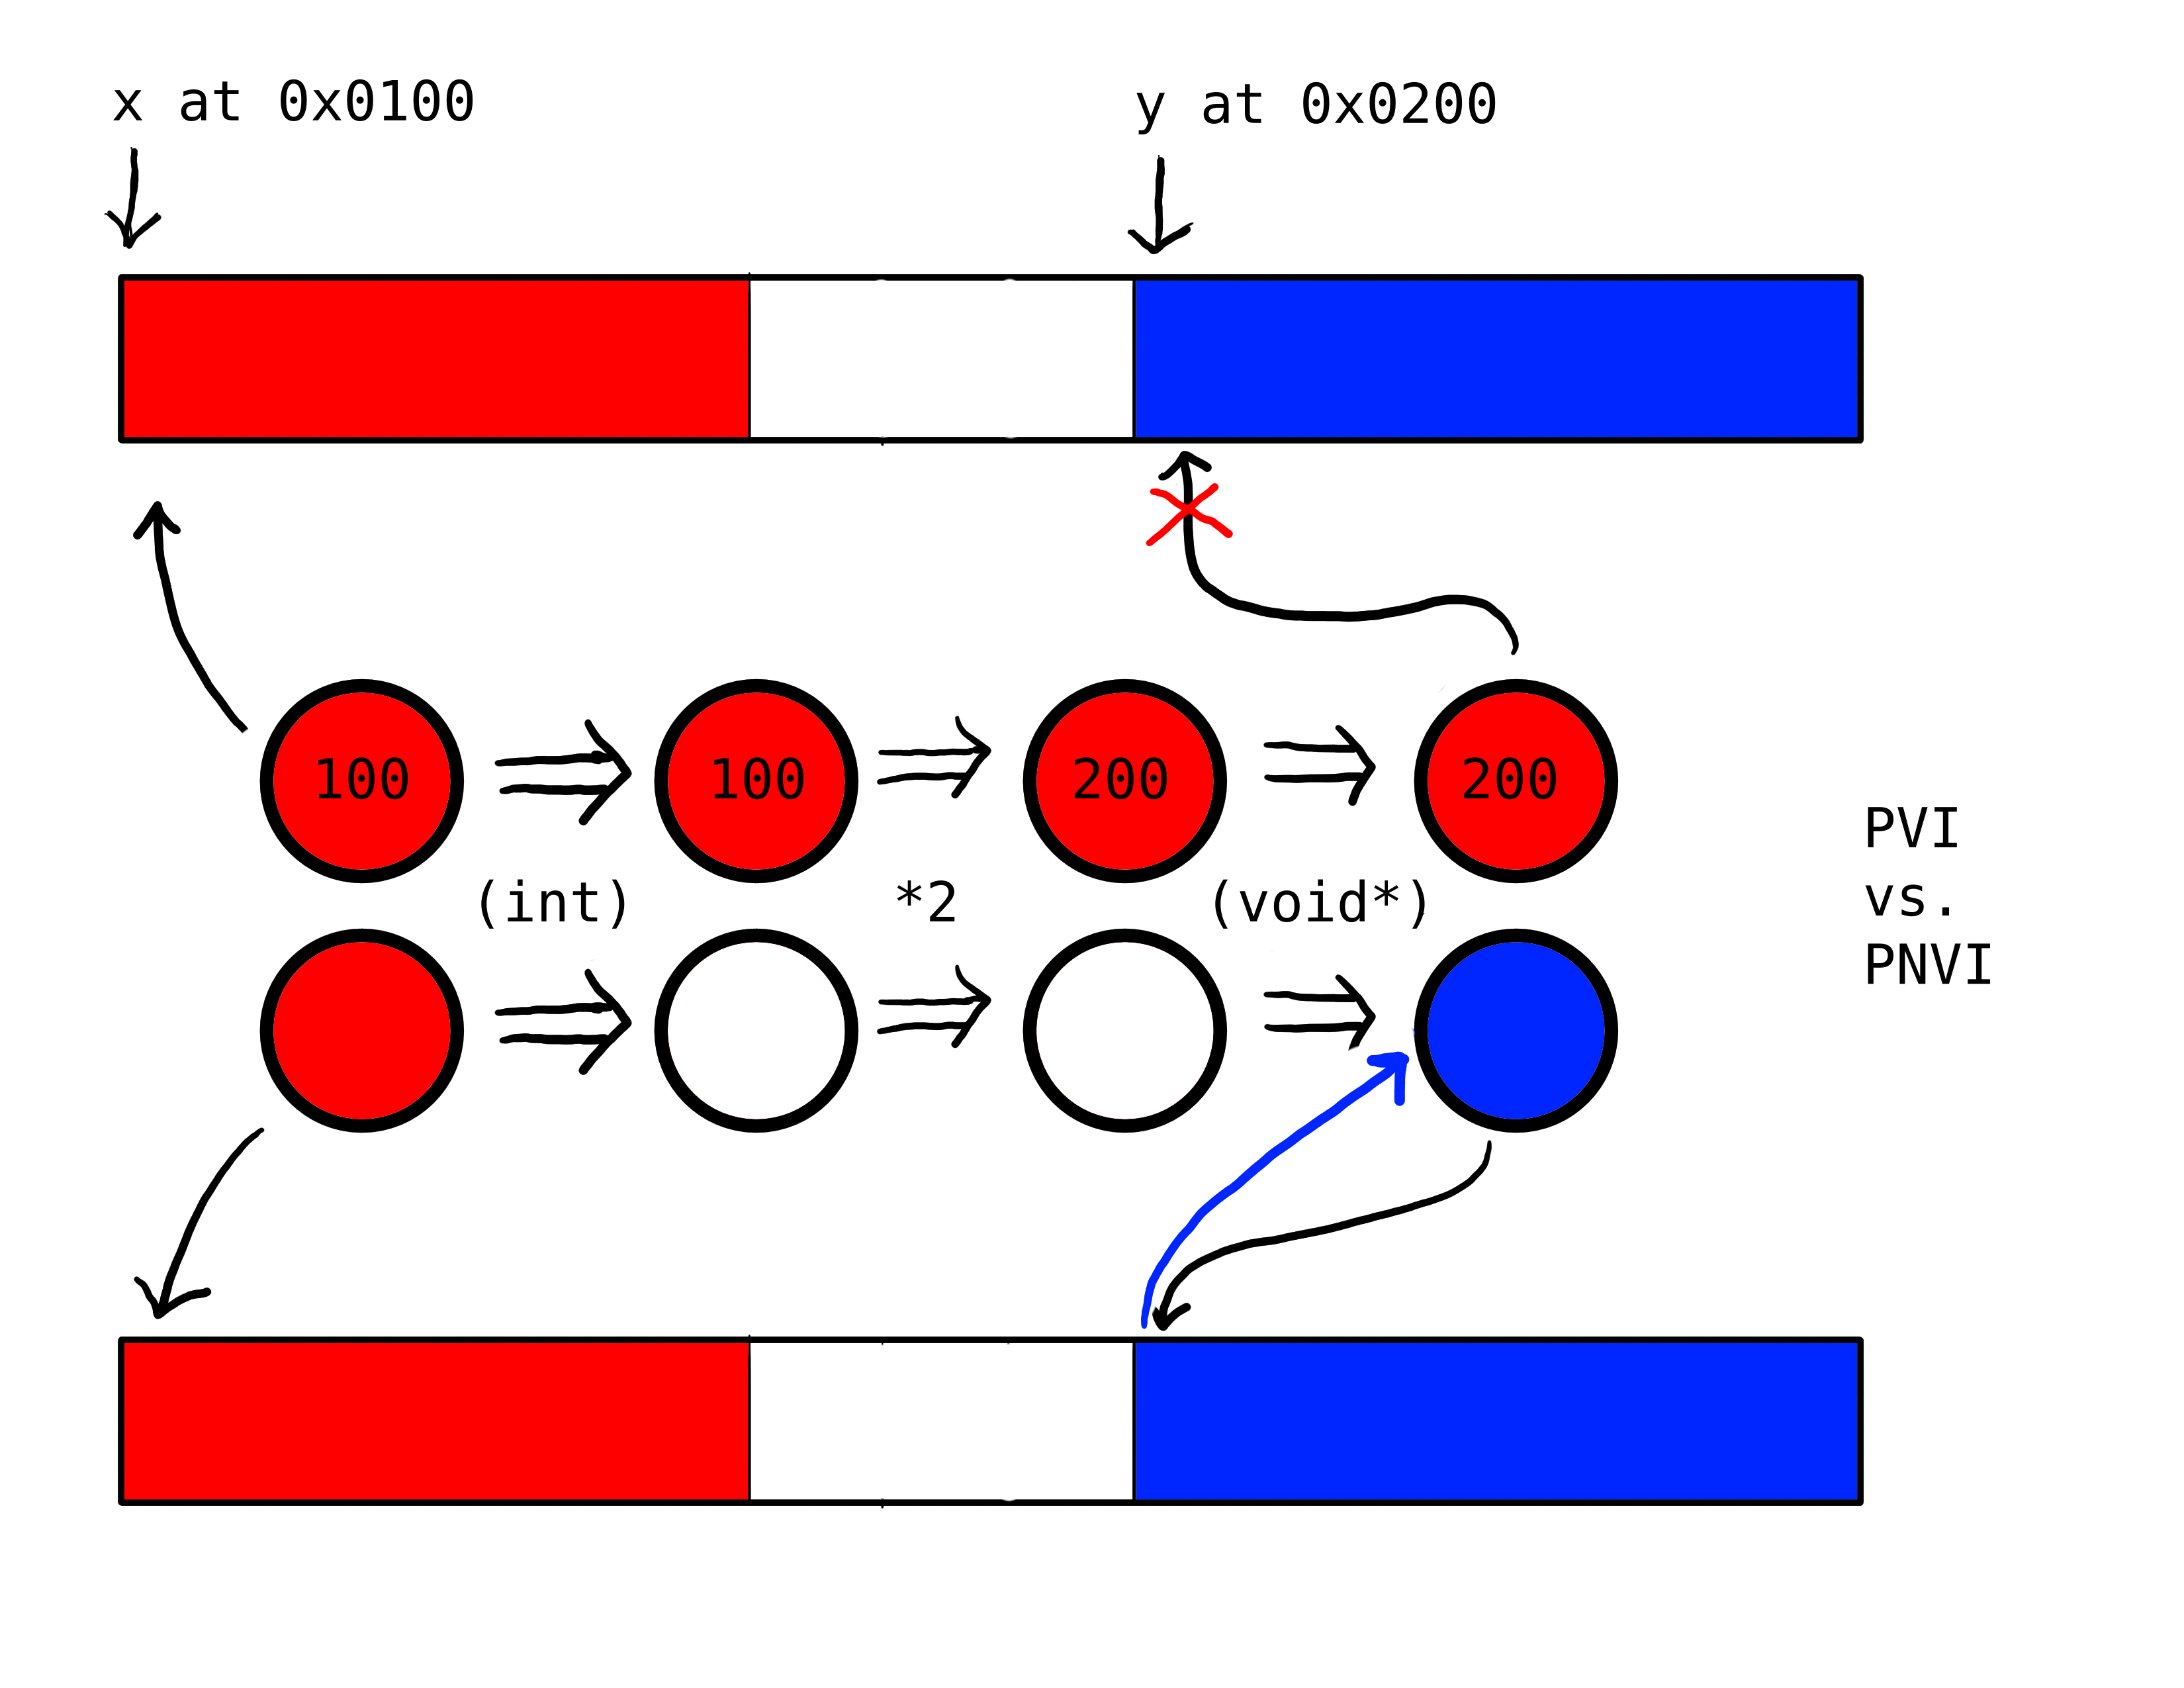
\includegraphics[width=.6\textwidth]{PVIvsPNVI.png}
  \caption{Integer-pointer casts in PVI and PNVI}
  \label{fig:PVI-PNVI}
\end{figure}

%We will aim to prove that for any program, if it is run in both the PVI semantics
%and in Tagged C with our PVI policy, it either produces identical output, or it is both
%undefined in the PVI semantics and failstops in Tagged C. Likewise for PNVI, except that
%some UB in PNVI is non-deterministic, and we only require that it failstop in an execution
%that would {\it reach} the UB.

In PNVI, the basic provenance model remains the same as PVI, so we can reuse most of the
same rules. The primary difference is what happens when we cast a pointer to an integer.
In PVI, tags are propagated as normal.
To support PNVI, we need the {\it cast} expression to update the tags of a pointer
being cast to an integer and vice versa. We add two special-case steps to reflect this.

\judgmenttwo{\optional{\(\mem[p]_{|ty|} = \_@\vt_2 @ \overline{\lt}\)}}
            {\(\trule{\picasttres}{\picastt}\)}
            {\(\defestate{\cast{int}{\val{p}{\pt}}}{\tptr{ty}} \longrightarrow
              \defestate{\val{p}{vt}}{int}\)}

\judgmenttwo{\optional{\(\mem[p]_{|ty|} = \_@\vt_2 @ \overline{\lt}\)}}
            {\(\trule{\ipcasttres}{\ipcastt}\)}
            {\(\defestate{\cast{int}{\val{p}{\pt}}}{\tptr{ty}} \longrightarrow
              \defestate{\val{p}{vt}}{int}\)}

For casting an integer to a pointer, we don't need the optional ``peek'' at the memory that it points to.
We simply clear the tag on the resulting integer. On the other hand, when casting back to a pointer,
we need to check the color of the object that it points to.

\begin{minipage}{0.34\textwidth}
\[\begin{aligned}
\truledef{\picastt}
\settag{\PCT'}{\PCT}
\settag{\vt}{N}
\end{aligned}\]
\end{minipage}
\begin{minipage}{0.65\textwidth}
\[\begin{aligned}
\truledef{\ipcastt}
\assert{\exists t . \forall \lt \in \overline{\lt} . \lt = t \land t \not = N}
\settag{\PCT'}{\PCT}
\settag{\pt}{t}
\end{aligned}\]
\end{minipage}

\paragraph{Realizing the Integer-Pointer Cast}

The pointer cast rules take as input the tags on the location pointed to by the
argument being cast. This requires the compiler to add extra instructions to retrieve that tag.
On RISCV, the sequence would be as follows, assuming that {\tt a0} contains the
value being cast. The meaning of instruction tags will be explained below.

\begin{verbatim}
lw a1 a0 0 @ RETRIEVE
sub a1 a1 a1 @ L
add a0 a1 a0 @ IPCAST
\end{verbatim}

In the underlying assembly, we use instruction tags to inform the low-level monitor
of the purpose of each instruction. {\tt RETRIEVE} indicates a special load
whose job is retrieve value and location tags from a location in memory. When it sees
a {\tt RETRIEVE} tag, the monitor allows the load even if it should failstop under the
Concrete C backstop policy. If the load should failstop, however, it is given a default
tag rather than the tags on the memory. A legal load recieves both the value and the location
tags.

The {\tt L} instruction tag simply denotes taking the left-operand's tag on the result of a
binary operation. In this case both operations are identical, but we still need to pick one.
Finally, the {\tt IPCAST} tag declares that this instruction should mimic the Tagged-C-level
rule.

\subsection{Secure Information Flow}
\label{sec:SIF}

Memory safety and compartmentalization are both aimed at preventing or mitigating
memory errors. But programs can be memory safe and still do insecure things! Consider the
following code, in which we have some error-handling code that writes to a log.

\begin{verbatim}
int checked_div(int a, int b) {
  if (a % b == 0) {
    return a / b;
  } else {
    fprintf(log, "%d should divide %d but doesn't\n", b, a);
    return 0;
  }
}

void main(int factor) {
  ...
  int key = read_and_parse(keyfile);
  
  int dividend = checked_div(key, factor);
  if (!dividend) {
    ...
  } else {
    ...
  }
}
\end{verbatim}

The {\tt checked\_div} function sometimes writes its arguments to a log,
which is reasonable enough, except when it's called with a key as an argument!
Suddenly we have keys being written to an unexpected and probably unprotected file.

This is an instance of problematic information-flow. The solution is to implement
a {\em secure information flow} (SIF) policy in Tagged C. SIF is a variant of
{\em information flow control} (IFC) described in the venerable Denning and Denning
\cite{Denning77:SecureInformationFlow}. At its simplest, if we classify inputs and outputs to
the program into secure (``high'') and public (``low'') classifications, then the
high inputs do not influence the low outputs. This generalizes to an arbitrary set
of security classes, but out first example is concerned with just two: the value
returned from {\tt read\_and\_parse} and the output to the log.
In our treatment of this example, we will describe a policy tailored to this particular
set of security classes.

\paragraph*{SIF Example Policy 1}

Let's assume that {\tt read\_and\_parse} is an {\em external} function---that is, we will not
model its internal behavior, so we know nothing about the value it returns. We can therefore
treat that value as an input, and track its influence through the system.

For this initial, simplified policy, we will assume that it is the only input that we care about,
so we have three possible tags: the default tag
\(\N\) represents values that are not tainted by the sensitive input, the tag
\(\vtaint{}\) represents values that have been influenced by {\tt read\_and\_parse}, and the tag
\(\pctaint{\overline{L}}\) carries a set of labels representing that
the current control-flow of the program is tainted (we will discuss this in detail
below.)

Initially, the PC Tag is \(\pctaint{\emptyset}\), and all values and memory locations are
tagged \(\N\). The taint tags are introduced at the external call to {\tt read\_and\_parse}.
At the same time, all external calls must check that they aren't leaking a tainted value!

\begin{minipage}{0.25\textwidth}
{ \color{blue}
  \begin{align*}
    \tau ::= & \N \\
    & \vtaint{} \\
    & \pctaint{\overline{L}} \\
\end{align*} }
\end{minipage}
\begin{minipage}{0.74\textwidth}
\[\begin{aligned}
\truledef{\extcallt}
\assert{\forall \vt \in \overline{\vt} . \vt = \N \land \PCT = \N}
\settag{\PCT'}{\PCT}
\settag{\vt'}{\caseof{f}}
\caseentry{read\_and\_parse}{\vtaint{}} \\
\caseentry{\_}{\vt} \\
\end{aligned}\]
\end{minipage}

When two values are combined with a binary operation, the resulting value is tainted
if either of them was. We define this as the {\em join} or {\em least-upper-bound}
operator, \(\sqcup\).

\begin{minipage}[t]{.49\textwidth}
\[t_1 \sqcup t_2 \triangleq
\begin{cases}
  \vtaint{} & \textnormal{if } t_1 = \vtaint{} \\
  \vtaint{} & \textnormal{if } t_2 = \vtaint{} \\
  \N & \textnormal{otherwise} \\
\end{cases}\]
\end{minipage}
\begin{minipage}[t]{.49\textwidth}
  \[\begin{aligned}
  \truledef{\binopt}
  \settag{\vt'}{
    \vt_1 \sqcup \vt_2
  }
  \end{aligned}\]
\end{minipage}

The policy needs to failstop if a tainted value becomes visible to the outside world.
That can happen when the value is passed as an argument to an external function, as we
saw above, or when it is stored to volatile memory (typically representing a file or external
device that might be read or might transfer. [TODO: need to introduce volatile memory earlier.]
%
\[\begin{aligned}
\truledef{\volstoret}
\assert{\PCT \sqcup \pt \sqcup \vt_2 = \N}
\settag{\PCT'}{\PCT}
\settag{\vt'}{\PCT \sqcup \pt \sqcup \vt_2}
\settag{\overline{\lt'}}{\overline{\lt}}
\end{aligned}\]

Now things become trickier, because the program's control-flow itself can be tainted.
This can occur in any of our semantics' steps that can produce different statements and continuations
depending on the tained value. At that point, any change to the machine state constitutes
an information flow. This is termed an {\em implicit flow}.

To be more specific, consider a statement that contains an expression, \(\stmt(\expr)\),
such that when filled in with a tainted value:
%
\[\sstate{\PCT}{\mem}{\stmt\val{v_1}{\mathit{taint} ~ \sigma}}{\cont} \longrightarrow
\sstate{\PCT_1}{\mem_1}{\stmt_1}{\cont_1}\]
%
while
%
\[\sstate{\PCT}{\mem}{\stmt\val{v_1}{\mathit{taint} ~ \sigma}}{\cont} \longrightarrow
\sstate{\PCT_2}{\mem_2}{\stmt_2}{\cont_2}\]
%
and where \(\stmt_1 \not = \stmt_2\) or \(\cont_1 \not = \cont_2\). Taking either step
should taint the program state itself! We represent this as a taint on the PC Tag.
When the PC Tag is tainted, all stores to memory and all updates to environments must
also be tainted until all branches eventually rejoin.
We term the point at which it is safe to remove taint a {\it join point}.
In terms of the program's control-flow graph, the
join point of a branch is its immediate post-dominator.

In many simple programs, the join point of a conditional or loop is obvious:
the point at which the chosen branch is complete, or the loop has ended.
Such a simple example can be seen in \cref{fig:ifthenelse}; {\tt public1} must be
tagged with the taint tag of {\tt secret}, while it is safe to tag {\tt public2}
\(\N\), because that is after the join point, {\tt J}. The same goes for \cref{fig:while},
because we are in a {\em termination-insensitive} setting \cite{}. This means that we
consider only terminating runs. So, we can guarantee that the post-dominator \(J\)
of the while loop is reached. [TODO: explain this more.]

But in the presence of unrestricted go-to statements, a join point may not be
local---and sometimes may not exist within the function, assuming that we have not
consolidated return points. Consider \cref{fig:forbreak}, which
uses go-to statements to create an approximation of an if-statement whose join-point
is far removed from the for-loop. The label {\tt J} now has nothing to do with the
semantics of any particular statement.

Luckily this can still be determined statically from a function's full
control-flow graph. So, to implement the policy, we must first transform our program
by adding labels at the join point of each conditional.
Every statement that branches carries an optional label indicating its corresponding
join point. If it doesn't have such
a label, that indicates that there is no join point within the function---once the PC Tag is tainted,
it must remain so until a return.

\begin{figure}
  \begin{subfigure}{0.5\textwidth}
\begin{verbatim}
int f(bool secret) {
    int public1, public2;

S:  if (secret) {
b1:     public1 = 1;
    } else {
b2:     public1 = 0;
    }

J:  public2 = 42;

    return public2;
}
\end{verbatim}
  \end{subfigure}
  \begin{subfigure}{0.5\textwidth}
    \begin{tikzpicture}
      [ initial text={}, initial distance=4em,
        accepting/.style=accepting by arrow,
        accepting distance=4em
      ]
      \node[state,initial]    (S)                        {$S$};
      \node[state]            (b_1) [above right=of S]   {$b_1$};
      \node[state]            (b_2) [below right=of S]   {$b_2$};
      \node[state,accepting]  (J)   [below right=of b_1] {$J$};

      \path[->] (S)   edge              node  {}  (b_1)
                      edge              node  {}  (b_2)
                (b_1) edge              node  {}  (J)
                (b_2) edge              node  {}  (J);
    \end{tikzpicture}
  \end{subfigure}
  
  \caption{Leaking via if statements}
  \label{fig:ifthenelse}
\end{figure}

\begin{figure}
  \begin{subfigure}{0.5\textwidth}
\begin{verbatim}
int f(bool secret) {
    int public1=1;
    int public2;

S:  while (secret) {
b1:     public1 = 1;
        secret = false;
    }

J:  public2 = 42;

    return public2;
}
\end{verbatim}
  \end{subfigure}
  \begin{subfigure}{0.5\textwidth}
    \begin{tikzpicture}
      [ initial text={}, initial distance=4em,
        accepting/.style=accepting by arrow,
        accepting distance=4em
      ]
      \node[state,initial]    (S)                        {$S$};
      \node[state]            (b_1) [above right=of S]   {$b_1$};
      \node[state,accepting]  (J)   [below right=of b_1] {$J$};

      \path[->] (S)   edge               node  {}  (b_1)
                      edge               node  {}  (J)
                (b_1) edge [bend right] node  {}  (S);
    \end{tikzpicture}
  \end{subfigure}
  
  \caption{Leaking via while statements}
  \label{fig:while}
\end{figure}

\begin{figure}
  \begin{subfigure}{0.25\textwidth}
\begin{verbatim}
int f(bool secret) {
    int public1, public2;

    while (secret) {
        goto b1;
    }

b2: public1 = 1;
    goto J;

b1: public1 = 1;

J:  public2 = 42;
    return public2;
}
\end{verbatim}
  \end{subfigure}
  \begin{subfigure}{0.74\textwidth}
    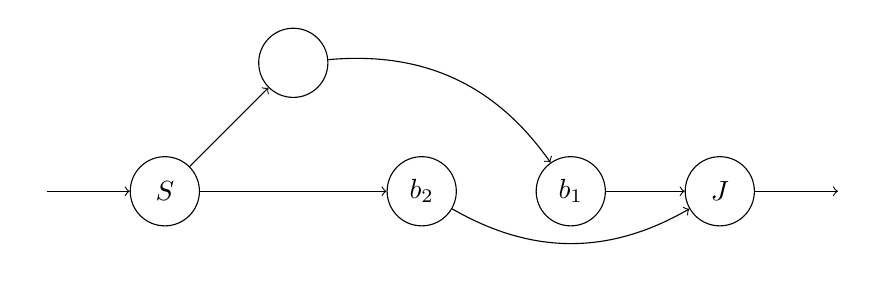
\begin{tikzpicture}
      [ initial text={}, initial distance=3em,
        accepting/.style=accepting by arrow,
        accepting distance=3em
      ]
      \node[state,initial]    (S)                              {$S$};
      \node[state]            (inside) [above right=of S]      {};
      \node[state]            (b_2)    [below right=of inside] {$b_2$};
      \node[state]            (b_1)    [right=of b_2]          {$b_1$};
      \node[state,accepting]  (J)      [right=of b_1]          {$J$};

      \path[->] (S)   edge              node  {}  (inside)
                      edge              node  {}  (b_2)
                (inside) edge [bend left] node {} (b_1)
                (b_1) edge              node  {}  (J)
                (b_2) edge [bend right] node  {}  (J);
    \end{tikzpicture}
  \end{subfigure}
  
  \caption{Cheating with go-tos}
  \label{fig:forbreak}
\end{figure}
\begin{figure}
  \begin{subfigure}{0.5\textwidth}
    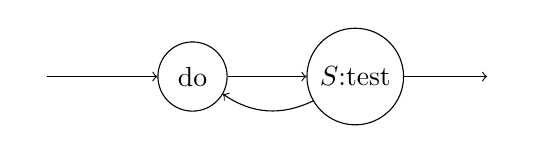
\begin{tikzpicture}
      [ initial text={}, initial distance=4em,
        accepting/.style=accepting by arrow,
        accepting distance=3em
      ]
      \node[state,initial]    (do)                             {do};
      \node[state,accepting]  (S) [right=of do]                {\(S\):test};

      \path[->] (do)   edge              node  {}  (S)
                (S)    edge [bend left]  node  {}  (do);
    \end{tikzpicture}
    \subcaption{Do-while}
  \end{subfigure}
  \begin{subfigure}{0.5\textwidth}
    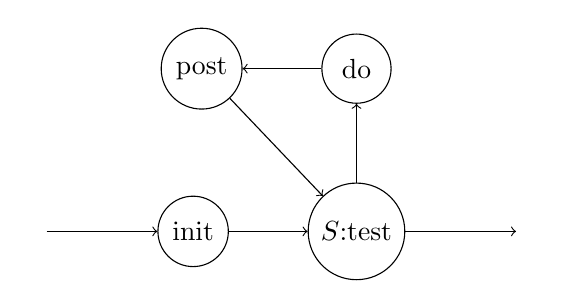
\begin{tikzpicture}
      [ initial text={}, initial distance=4em,
        accepting/.style=accepting by arrow,
        accepting distance=4em
      ]
      \node[state,initial]    (init)                             {init};
      \node[state,accepting]  (S)    [right=of init]             {\(S\):test};
      \node[state]            (do)   [above=of S]                {do};
      \node[state]            (post) [left=of do]                {post};
      
      \path[->] (init)   edge              node  {}  (S)
                (S)      edge              node  {}  (do)
                (do)     edge              node  {}  (post)
                (post)   edge              node  {}  (S);
    \end{tikzpicture}
    \subcaption{For}
  \end{subfigure}
  \begin{subfigure}{\textwidth}
    \center
    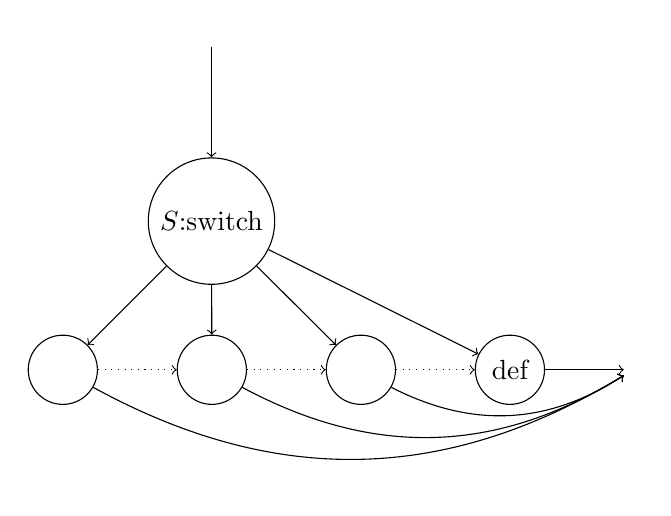
\begin{tikzpicture}
      [ initial text={}, initial distance=4em, initial above,
        accepting/.style=accepting by arrow,
        accepting distance=4em
      ]
      \node[state,initial]    (switch)                           {\(S\):switch};
      \node[state]            (case1)    [below left=of switch]  {};
      \node[state]            (case2)    [right=of case1]        {};
      \node[state]            (case3)    [right=of case2]        {};
      \node[state]            (default)  [right=of case3]        {def};
      \node                   (after)    [right=of default]      {};

      \path[->] (switch)  edge              node  {}  (case1)
                          edge              node  {}  (case2)
                          edge              node  {}  (case3)
                          edge              node  {}  (default)
                (default) edge              node  {}  (after)
                (case1)   edge [bend right] node  {}  (after)
                (case2)   edge [bend right] node  {}  (after)
                (case3)   edge [bend right] node  {}  (after);

      \path[dotted,->] (case1) edge              node  {}  (case2)
                (case2) edge              node  {}  (case3)
                (case3) edge              node  {}  (default);
                         
    \end{tikzpicture}
    \subcaption{Switch}
  \end{subfigure}
  
  \caption{Remaining Branch Statements}
  \label{fig:rest}
\end{figure}

\paragraph*{Intransitive SIF}

Our second example involves information from outside of the system ending up somewhere it isn't supposed to.

\begin{verbatim}
void sanitize(src, dst);
char* sql_query(char* query);

void get_data(char* name, char* buf, int field) {
  // field: 1=address, 2=phone, 3(default)=astrological sign
  char[10] name_san;
  char[100] query;
  sanitize(name, name_san);

  switch(field) {
    case 1:
      sprintf(query, "select address where name =");
      strncat(query, name_san, strlen(name_san));
      break;
    case 2:
      sprintf(query, "select phone where name =");
      strncat(query, name_san, strlen(name_san));
      break;
    default:
      sprintf(query, "select sign where name =");
      strncat(query, name, strlen(name)); // Oops!
      break;
  }

  sprintf(buf, sql_query(query);
  return;
}
\end{verbatim}

This function sanitizes its input {\tt name}, then appends the result to an appropriate SQL
query, storing the result in {\tt buf}. But, in the default case, the programmer has accidentally
used the unsanitized string! This creates the opportunity for an SQL injection attack: a caller
to this function could (presumably at the behest of an outside user) call it with {\tt field} of
3 and {\tt name} of ``Bobby; drop table;''.

In the second example, we particularly want to implement an {\it intransitive} SIF policy:
we wish to allow {\tt name} to influence the result of {\tt sanitize}, naturally, and the result
of {\tt sanitize} to influence the value passed to {\tt sql\_query}, but we do not wish for
{\tt name} to influence {\tt sql\_query} directly.

\paragraph*{Tracking Data Sources and Sinks}

The core of our SIF policies is that we identify parts of the state as {\em sources} and as {\em sinks}.
A source \(\sigma\) can be an argument of a function, its return value, or a global.
A sink \(\psi\) can be any of these, plus the set of heap objects allocated by a given function.
We write them as follows:

\begin{minipage}{0.5\textwidth}
  \[\begin{aligned}
  \sigma ::= & x & \textnormal{Global} \\
  & f(x) & \textnormal{Argument {\tt x} of {\tt f}} \\
  & f.ret & \textnormal{Return value of {\tt f}} \\
  \end{aligned}\]
\end{minipage}
\begin{minipage}{0.5\textwidth}
  \[\begin{aligned}
  \psi ::= & x & \textnormal{Global} \\
  & f(x) & \textnormal{Argument {\tt x} of {\tt f}} \\
  & f.ret & \textnormal{Return value of {\tt f}} \\
  & f.m & \textnormal{Memory owned by {\tt f}} \\
  \end{aligned}\]
\end{minipage}

We track the influence of a particular source, or its ``taint,'' through the system in the form
of tags on values. Sinks that are in memory have their memory locations tagged accordingly. And
the PC Tag at all times tracks a set of sources that are implicitly influencing the state, described
further below.
%
\begin{align*}
  \tau ::= & \mathit{vtaint} ~ \overline{\sigma} \\
  & \mathit{sink} ~ \psi \\
  & \mathit{pctaint} ~ \overline{(L,\sigma)} \\
\end{align*}
%


%In classic SIF theory, we specify an {\em information flow policy} (IFPol)---not to be confused with a
%tag policy---as a relation \(\cdot \rightsquigarrow \cdot \in \sigma \times \psi\). However,
%manually defining such a policy is challenging, especially in an intransitive setting.
%We envision the IFPol being initially stated in negative terms, with the ``no-flow'' relation
%\(\not \rightsquigarrow\). That is, we will assume by default that for any source \(\sigma\)
%and any sink \(\psi\), \(\sigma \rightsquigarrow \psi\), unless the user has explicitly
%declared the contrary.

%So, in the above example, the user would declare that \(\mathtt{name} \not \rightsquigarrow \mathtt{sql\_query}\).
%But, in the case of \(\mathtt{sanitize}\), we want it to be the case that \(\mathtt{name}\) can flow to
%\(\mathtt{sql\_query}\) only via \(\mathtt{sanitize}\). We therefore need to allow the user to declare
%a {\em declassification} rule. In general we will write \(\sigma / \sigma'\) to indicate that \(\sigma'\)
%supersedes \(\sigma\): if a value that has been influenced by \(\sigma\) influences \(\sigma'\), we
%can safely ignore its history with \(\sigma\). We may write \(* / \sigma\) to say that \(\sigma\)
%declassifies anything.

%For example, suppose that in the following code, we want to enforce a no-flow rule between
%the argument {\tt x} of {\tt f} and the global variable {\tt z}
%(\(\mathtt{f.x} \not \rightsquigarrow \mathtt{z}\)), and a declassification rule
%\(* / \mathtt{g.a}\).

%\begin{verbatim}
%  int z;
%
%  int g(int a);
%
%  void f(int x, int y) {
%    z = x;                    // violation
%    z = x + y;                // violation
%    if(x) z = 1; else z = 0;  // violation
%    z = g(x);                 // violation, unless f.x / g.a
%  }
%\end{verbatim}

%The first three lines of {\tt f} violate the no-flow relation by storing values derived from
%{\tt x} into {\tt z}. The third line is especially interesting: although {\tt x} is not stored
%directly, the value that is stored is conditioned upon it, and can be used to deduce information
%about the original value. This is termed an {\em implicit flow}. Finally, in the last line,
%the value of {\tt g(x)} depends on {\tt x}, which is a violation unless it is subject to a
%declassification rule.

%We can therefore define an IFPol as a set of rules of each kind:

%\[I \subseteq \{\sigma \not \rightsquigarrow \psi \mid \sigma \not \eq \psi\} \cup
%\{\sigma / \sigma' \mid \sigma \not \eq \sigma'\}\]

%We do not need to distinguish between rules that notionally represent ``integrity'' versus ``confidentiality''
%concerns. The SQL injection example is an instance of integrity, ensuring that an input cannot influence data
%in an undesired way, but the same concept can be used to prevent data from influencing the program's output
%inappropriately.

%\paragraph{SIF, formally}

%We can characterize the protection offered by a SIF policy in terms of a {\em non-interference}
%property along the lines of Bay and Askarov \cite{}. We annotate our transitions with events \(\alpha\),
%each representing the transmission of a value through a source or sink---possibly several. We write the
%projection of data relevant to a particular source \(\sigma\) or sink \(\psi\) as \(\pi_\sigma(\alpha)\)
%or \(\pi_\psi(\alpha)\).

%\[\begin{aligned}
%\alpha ::= & \\
%& \\
%\end{aligned}\]

%[TODO: add the relevant events to their transitions in the semantics, and list them here.]

%Now, we define the knowledge that an observer monitoring a particular sink can extrapolate about the
%state of the system as a whole, as a set of states that are consistent with the events it observes.
%Given some initial state \(S\), this is precisely the set of other initial states that might
%produce the same trace (or an extension thereof) and that are equivalent.

%\[\mathbf{K}(S,\overline{\alpha},\sigma,\psi) \triangleq
%\{S' \mid S \sim_\sigma S' \land S' \hookrightarrow_{\psi} \overline{\alpha} \cdot \alpha\}\]

%Then, absent any declassification rules, we can define non-interference as holding between
%\(\sigma\) and \(\psi\) if, for any states \(S_1\) and \(S_2\) such that
%\(S_1 \xrightarrow{\overline{\alpha}\cdot \alpha} S_2\),
%\(\mathbf{K}(S_2,\overline{\alpha}\cdot \alpha,\sigma,\psi) \supseteq
%\mathbf{K}(S_1,\overline{\alpha},\sigma,\psi)\). That is, every world that was possible before
%\(\alpha\) remains possible after.

%In the presence of declassification, we add an exception for the case where \(\alpha\)
%reflects an event that should indeed allow an observer to gain some information. We extend
%the above definition to talk about all of \(I\).

%\[NI_I \triangleq \forall S_1, S_2, \overline{\alpha}, \alpha .
%\begin{cases}
%\mathbf{K}(S_2,\overline{\alpha}\cdot \alpha,\sigma,\psi) \supseteq
%\mathbf{K}(S_1,\overline{\alpha},\sigma,\psi) &
%\textnormal{if } \sigma \not \rightsquigarrow \psi \in I \\
%\mathbf{K}(S_2,\overline{\alpha}\cdot \alpha,\sigma,\psi) \supseteq
%\mathbf{K}(S_1,\overline{\alpha},\sigma \sqcup \sigma',\psi &
%\textnormal{if } \sigma / \sigma' \in I \land \sigma' \rightsquigarrow \psi \in I \\
%\end{cases}\]

A value that is tagged \(\mathit{vtaint} ~ \overline{\sigma}\) has been influnced
by all of the sources in \(\overline{\sigma}\). We also define a set of tags that indicate that a
particular function argument or the memory location of an object represents a sink that is the
target of one or more no-flow rules. If a sink \(\psi\) is tagged
\(\mathit{forbid} ~ \overline{\sigma}\), then for all \(\sigma \in \overline{\sigma}\),
\(\sigma \not \rightsquigarrow \psi\) must be in our IFPol. Finally, the PC Tag must carry additional
information: when the PC Tag is tainted, it must keep a record of the scope of the taint, in the form
of a label. We will explain below how this scope is computed.
%
%
We define four important operations on tags: {\em join} (\(t_1 \sqcup t_2\)), {\em bounded join}
(\(t_1 [L \rightarrowtail t_2]\)), {\em minus} (\(t_1 - t_2\)), and {\em check} (\(t_1 \models t_2\)),
all partial functions.
%
\[t_1 \sqcup t_2 \triangleq
\begin{cases}
  \mathit{vtaint} ~ (\overline{\sigma}_1 \cup \overline{\sigma}_2) &
  \textnormal{if } t_1 = \mathit{vtaint} ~ \overline{\sigma}_1 \textnormal{ and }
  t_2 = \mathit{vtaint} ~ \overline{\sigma}_2\\
  \mathit{vtaint} ~ (\overline{\sigma}_2 \cup \{\sigma \mid (L,\sigma) \in \overline{(L,\sigma)}_1\}) &
  \textnormal{if } t_1 = \mathit{pctaint} ~ \overline{(L,\sigma)}_1 \textnormal{ and }
  t_2 = \mathit{vtaint} ~ \overline{\sigma}_2\\
  \mathit{vtaint} ~ (\overline{\sigma}_1 \cup \{\sigma \mid (L,\sigma) \in \overline{(L,\sigma)}_2\}) &
  \textnormal{if } t_2 = \mathit{pctaint} ~ \overline{(L,\sigma)}_2 \textnormal{ and }
  t_1 = \mathit{vtaint} ~ \overline{\sigma}_1\\
  \bot & \textnormal{otherwise} \\
\end{cases}\]
%
\[L \rightarrowtail t_1 \sqcup t_2 \triangleq
\begin{cases}
  \mathit{pctaint} ~ (\overline{\sigma}_1 \cup \overline{\sigma}_2) &
  \textnormal{if } t_1 = \mathit{vtaint} ~ \overline{\sigma}_1 \textnormal{ and }
  t_2 = \mathit{vtaint} ~ \overline{\sigma}_2\\
  \bot & \textnormal{otherwise} \\
\end{cases}\]
%
\[t - \sigma \triangleq
\begin{cases}
  \mathit{taint} ~ (\overline{\sigma}' - \sigma) &
  \textnormal{if } t = \mathit{taint} ~ \overline{\sigma}' \\
  \bot & \textnormal{otherwise} \\
\end{cases}\]
%
\[t_2 \models t_1 \triangleq
\begin{cases}
  \mathbf{t} & \textnormal{if } t_1 = \mathit{taint} ~ \overline{\sigma}_1,
  t_2 = \mathit{forbid} ~ \overline{\sigma}_2, \textnormal{ and }
  \overline{\sigma}_1 \cap \overline{\sigma}_2 = \emptyset \\
  \mathbf{f} & \textnormal{if } t_1 = \mathit{taint} ~ \overline{\sigma}_1,
  t_2 = \mathit{forbid} ~ \overline{\sigma}_2, \textnormal{ and }
  \overline{\sigma}_1 \cap \overline{\sigma}_2 \not = \emptyset \\
  \bot & \textnormal{otherwise} \\
\end{cases}\]

\paragraph{Tainting and Checking Arguments and Returns}

Now we can begin to give our policy, given an arbitrary IFPol \(I\).

A function argument or return value can be either a source or a sink.
So, when they are processed by the {\em call-state} and {\em return-state} rules,
we must both check that the value being passed or returned is not tainted by a forbidden
source, and then add the current source to its taint.
The call-state rule executes at the beginning of a call, moving all of its arguments into
the local environment, using the \(\mathbf{ArgT}\) tag rule.
The return-state rule executes after the call returns, inserting the result into the
context saved in the continuation. The program counter on return and the result's tag are
set by the \(\mathbf{rettname}\) tag rule. Both are given in \cref{fig:callretsteps}.

\begin{figure}
  \callstep
  \returnstep
  \caption{Call and Return Steps}
  \label{fig:callretsteps}
\end{figure}
  
\begin{minipage}[t]{.49\textwidth}
  \[\begin{aligned}
  \truledef{\argt}
  \letin{t := \mathit{forbid} ~ \{\sigma \mid \sigma \not \rightsquigarrow f(x) \in I\}}
  \assert{t \models \PCT \sqcup \vt}
  \letin{\vt_1 := \vt - \{\sigma \mid \sigma / f(x) \in I \}}
  \letin{\vt_2 := \vt_1 \sqcup \mathit{tainted} ~ \{f(x)\}}
  \settag{\vt'}{\vt_2}
  \end{aligned}\]
\end{minipage}
\begin{minipage}[t]{.49\textwidth}            
  \[\begin{aligned}
  \truledef{\rett}
  \letin{t := \mathit{forbid} ~ \{\sigma \mid \sigma \not \rightsquigarrow f.ret \in I\}}
  \assert{t \models \PCT \sqcup \vt}
  \letin{\vt_1 := \vt - \{\sigma \mid \sigma / f.ret \in I \}}
  \letin{\vt_2 := \vt_1 \sqcup \mathit{tainted} ~ \{f.ret\}}
  \settag{\vt'}{\vt_2}
  \end{aligned}\]
\end{minipage}

Global variables are also possible sources or sinks. In this case, we initialize their
tags to carry this information.
\[\begin{aligned}
\truledef{\globalt}
\settag{\pt}{\mathit{tainted} ~ \emptyset}
\settag{\vt}{\mathit{tainted} ~ \{x\}}
\settag{\overline{\lt}}{\left[\mathit{forbidden} ~ \{\sigma \mid x \not \rightsquigarrow x \in I\}\right]}
\end{aligned}\]

\paragraph{Introducing Dynamic Sinks}

One scenario that does not really match the others is when the sink is dynamically allocated
memory. In this case, we need to tag the memory at allocation-time with the forbidden
sources.

\[\begin{aligned}
\truledef{\malloct}
\settag{\pt}{\PCT \sqcup \mathit{tainted} ~ \emptyset}
\settagopt{\vt}{\mathit{tainted} ~ \emptyset}
\settagopt{\overline{\lt}}{\left[\mathit{forbidden} ~ \{\sigma \mid \sigma \not \rightsquigarrow f.m\} \right]}
\settag{\PCT'}{\PCT + 1}
\end{aligned}\]

\paragraph{Propagating Taint Through Expressions}

It is simple enough to determine when a value is tainted: at a function
call, all function arguments are tagged with their source identity, and the result
of any expression is tagged with the union of the sources of its operands. If the
expression involves a store or function call itself, we must check the taints on
the value being stored or passed against the forbidden list of the target.

Unary and binary operations:

\begin{minipage}[t]{.49\textwidth}
  \[\begin{aligned}
  \truledef{\unopt}
  \settag{\vt'}{\vt}
  \end{aligned}\]
\end{minipage}
\begin{minipage}[t]{.49\textwidth}
  \[\begin{aligned}
  \truledef{\binopt}
  \settag{\vt'}{
    \vt_1 \sqcup \vt_2
  }
  \end{aligned}\]
\end{minipage}

Loads and stores:

\begin{minipage}[t]{.4\textwidth}
\[\begin{aligned}
\truledef{\loadt}
\settag{\vt'}{\PCT \sqcup \pt \sqcup \vt}
\end{aligned}\]
\end{minipage}
\begin{minipage}[t]{.59\textwidth}
\[\begin{aligned}
\truledef{\storet}
\assert{\forall \lt \in \overline{\lt} . \lt \models \PCT \sqcup \pt \sqcup \vt_2}
\settag{\PCT'}{\PCT}
\settag{\vt'}{\PCT \sqcup \pt \sqcup \vt_2}
\settag{\overline{\lt'}}{\overline{\lt}}
\end{aligned}\]
\end{minipage}

\begin{figure}
  \ifstepb
  
  \whiletruestep
  \whilefalsestep
  \whileskipcontinuestep
  \whilebreakstep

  \labelstep

  \caption{Selected Conditional Steps}
  \label{fig:conditionals}
\end{figure}


When we step into a conditional or loop, we record its join point on the PC Tag, associated with the sources
that are tainted. Then, when we reach the label, we will subtract its sources from the PC Tag at that time.
This means that if multiple branches share a join point, their taints will be removed simultaneously.

\begin{minipage}[t]{.25\textwidth}
\[\begin{aligned}
\truledef{\splitt}
\settag{\PCT'}{\PCT[L \rightarrowtail \vt]}
\end{aligned}\]
\end{minipage}
\begin{minipage}[t]{.74\textwidth}
\[\begin{aligned}
\truledef{\labelt}
\assert{\PCT = \mathit{pctaint} ~ \overline{(L,\sigma)}\}}
\settag{\PCT'}{\mathit{pctaint} ~ \{(L',\sigma) \mid (L',\sigma) \in \overline{(L,\sigma)} \land L \not \eq L'\}}
\end{aligned}\]
\end{minipage}

The \(\labeltname\) control point applies whenever we reach a labeled statement, seen
in \cref{fig:conditionals}.
The remaining branching constructs are rather complicated, involving multiple steps
and manipulations of the continuation that are not that relevant to their control
points. Rather than give their semantics in full, it suffices to identify which
transitions contain \(\mathbf{SplitT}\) control points. In \cref{fig:rest}, these
are the transitions from the state marked \(S\). Their semantics are given in full
in the appendix.

\paragraph*{Realizing IFC}

In order to implement an IFC policy, we need to specify the rules that it needs to enforce.
The positive here is that the rules are not dependent on one another (with the exception of
declassification rules), and default to permissiveness when no rule is given. We assume that
the user would supply a separate file consisting of a list of triples: the source, the sink,
and the type of rule. This is then translated into the policy.

The other implementation detail to consider are the label tags. These resemble
instruction tags, and that is exactly how they would be implemented: as a special instruction
tag on the appropriate instruction, which might be an existing instruction or a specially
added no-op. But importantly, in this case, these tags are mutable; in a policy that can be
expected to take advantage of their mutability, we will need an extra store to set the tag
for later.

It remains to generate those labels. For purposes of an IFC policy, we first generate the program's
control flow graph. Then, for each if, while, do-while, for, and switch statement, we identify the
immediate post-dominator in the graph, and wrap it in a label statement with a fresh identifier.
That identifier is also added as a field in the original conditional statement. The tags
associated with the labels are initialized at program state---in the case of IFC, these defaults
declare that there are no secrets to lowre when it is reached.

\section{Evaluation}
\label{sec:evaluation}

Tagged C aims to combine the flexibility of tag-based architectures with the abstraction
of a high-level language. How well have we achieved this aim?

[Here we list criteria and evaluate how we fulfilled them]

\begin{itemize}
\item Flexibility: we demonstrate three policies that can be used alone or in conjunction
\item Applicability: we support the full complement of C language features and give definition
  to many undefined C programs
\item Practical security: our example security policies are based on important security concepts
  from the literature
\end{itemize}

\subsection{Limitations of the Tag Mechanism}

By committing to a tag-based mechanism, we do restrict the space of policies that Tagged C
can enforce. In general, a reference monitor can enforce any policy that constitutes a
{\em safety property}---any policy whose violation can be demonstrated by a single finite
trace. This class includes such policies as ``no integer overflow'' and ``pointers are always in-bounds,''
which depend on the values of variables. Tag-based monitors cannot enforce any policy that
depends on the value of a variable rather than its tags.

\section{Future Work}
\label{sec:futurework}

We have presented the language and a reference interpreter, built on top of the CompCert interpreter
\cite{Leroy09:CompCert}, and three example policies. There are several significant next-steps.

\paragraph{Compilation}

An interpreter is all well and good, but a compiler would be preferable for many reasons.
A compiled Tagged C could use the hardware acceleration of a PIPE target, and could more easily
support linked libraries, including linking against code written in other languages.
The ultimate goal would be a fully verified compiler, but that is a very long way off.

\paragraph{Language Proofs}

There are a couple of properties of the language semantics itself that we would like to prove.
Namely (1) that its behavior (prior to adding a policy) matches that of CompCert C and
(2) that the behavior of a given program is invariant under all policies up to truncation due
to failstop.

\paragraph{Policy Correctness Proofs}

For each example policy discussed in this paper, we sketched a formal specification for the
security property it ought to enforce. A natural continuation would be to prove the correctness
of each policy against these specifications.

\paragraph{Policy DSL}

Currently, policies are written in Gallina, the language embedded in Coq. This is fine for a
proof-of-concept, but not satisfactory for real use. We plan to develop a domain-specific policy
language to make it easier to write Tagged C policies.

\bibliography{taggedc.bib}

\appendix

\section{Continuations}
\label{app:continuations}

\[\begin{split}
\cont ::= & \kemp \\
| & \kdo{\cont} \\
| & \kseq{\stmt}{\cont} \\
| & \kif{\stmt_1}{\stmt_2}{L}{\cont} \\
| & \kwhiletest{\expr}{\stmt}{L}{\cont} \\
| & \kwhileloop{\expr}{\stmt}{L}{\cont} \\
| & \kdowhiletest{\expr}{\stmt}{L}{\cont} \\
| & \kdowhileloop{\expr}{\stmt}{L}{\cont} \\
| & \kfor{\stmt}{\cont} \\
| & \kforpost{\stmt}{\cont} \\
\end{split}\]

\section{Initial State}

Given a list \(xs\) of variable identifiers \(id\) and types
\(ty\), a program's initial memory is defined by iteratively allocating each one
in memory and updating the global environment with its base address, bound, type,
and a static identity tag. Let \(|ty|\) be a function from types to their sizes
in bytes. The memory is initialized \(\vundef@\vt@\overline{\lt}\)
for some \(\vt\) and \(\overline{\lt}\), unless given an initializer.
Let \(\mem_0\) and \(\genv_0\) be the initial (empty) memory and environment.
The parameter \(b\) marks the start of the global region.

%Since we don't need to initialize tags in memory dynamically, our rule for
%selecting these tags can cover the entire initialization of the memory with arbitrary
%granularity. We represent this as a list of tags of length \(|ty|\).

\[\mathit{globals} ~ xs ~ b =
\begin{cases}
  (\mem_0, \genv_0) & \textnormal{if } xs = \varepsilon \\
  (\mem[p \dots p+|ty| \mapsto \vundef@\vt@\overline{\lt}]_{|ty|}, & \textnormal{if } xs = (id,ty)::xs' \\
  ~ \genv[id \mapsto (\mathit{p, p+|ty|,ty,\pt})]) & \textnormal{and } \trule{\globaltres}{\globalt} \\
  & \textnormal{where } (\mem,\genv) = \mathit{globals} ~ xs' ~ (b + |ty|) \\
\end{cases}\]

\section{Step rules}
\label{app:rules}

\subsection{Sequencing rules}

\dostepa
\dostepb
\seqstep
\seqskipstep
\seqcontinuestep
\seqbreakstep
\retvalstep
\labelstep

\subsection{Conditional rules}

\ifstepa
\ifstepb

TODO: switch

\subsection{Loop rules}

%% While %%
\whilestep
\whiletruestep
\whilefalsestep
\whileskipcontinuestep
\whilebreakstep

%% Do-while %%
\dowhilestep
\dowhileskipcontinuestep
\dowhilefalsestep
\dowhiletruestep
\dowhilebreakstep

%% For %%
\forinitstep
\forstep
\forfalsestep
\fortruestep
\forskiporcontinuestep
\forbreakstep
\forskippoststep

\subsection{Expression Rules}

\mallocstep
\valofstep
\assignopstep
\postincstep
\assignstep
\varstep
\unopstep
\binopstep
\callexprstep

\subsection{Call and Return Rules}

\[\mathit{locals} ~ xs ~ \mem ~ \lenv =
\begin{cases}
  (\mem, \lenv) & \textnormal{if } xs = \varepsilon \\
  \mathit{locals} ~ xs' ~ \mem'' ~ \lenv' & \textnormal{if } xs = (id,ty)::xs' \\
  & \textnormal{where } (\mem',p) \leftarrow \mathit{stack\_alloc} ~ |ty| ~ \mem, \\
  & \mem'' = \mem'[p \dots p+|ty| \mapsto \vundef@\vt@\overline{\lt}]_{|ty|}, \\
  & \trule{\localtres}{\localt}, \\
  & \textnormal{and } \lenv' = \lenv[id \mapsto (\mathit{p, p+|ty|,ty,\pt})]) \\
\end{cases}\]

\callstep
\returnstep

\subsection{Memory safety (old)}

Memory safety policies operate on under a ``lock and key'' model, in which objects in memory
are tagged with a unique identifier (the ``lock'') and may only be accessed via a pointer tagged
with the same identifier (the ``key.'') For a simple example, consider the following code:
%
\vspace{\abovedisplayskip}
\begin{verbatim}
void main() {
  int a[10];
  int b[10];
  a[10] = 42;    
}
\end{verbatim}
\vspace{\belowdisplayskip}
%
In a typical stack allocator---such as the one used by my interpreter---{\tt a} and {\tt b} will
be allocated next to one another on the stack, like this:

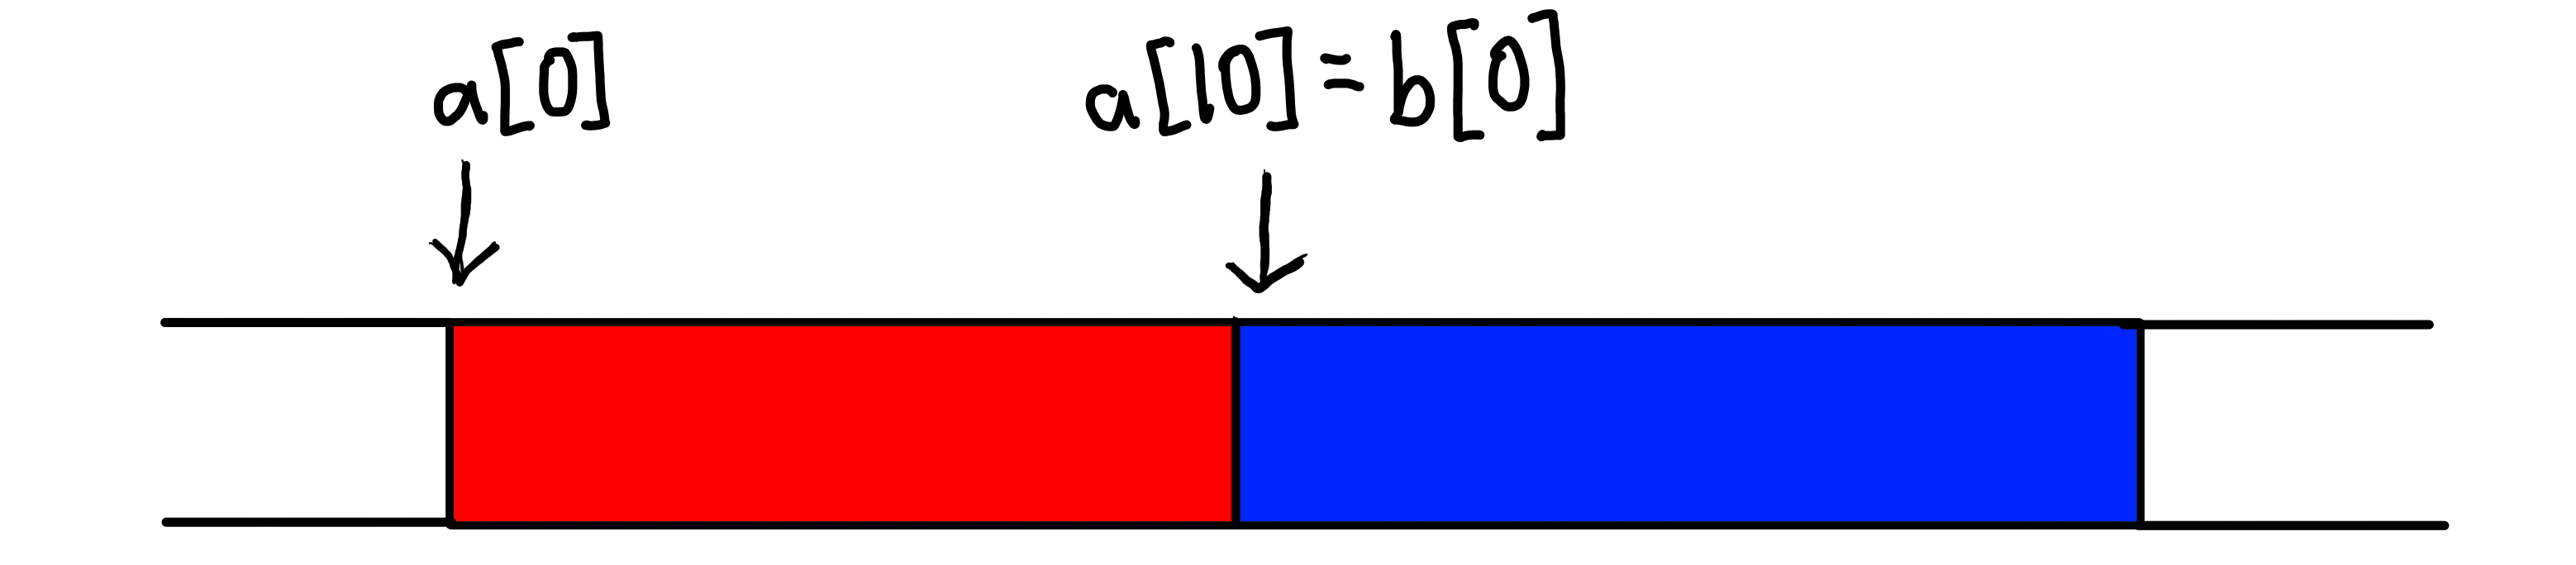
\includegraphics[width=.5\textwidth]{example.png}

To prevent the expression {\tt a[10] = 42} from overwriting {\tt b[0]}, we give {\tt a} and {\tt b}
unique {\it color tags} when they are allocated. In this case, we'll tag {\tt a} with \(\mathit{dyn ~ 0}\),
indicating that it's the first dynamically allocated object, and {\tt b} with \(\mathit{dyn ~ 1}\).
Then, when we evaluate the left-hand expression {\tt a} into its memory location \(l\), we tag
\(l\) with \(\mathit{dyn ~ 0}\). When we take the offset \(l + 10\), we keep that tag. And when we
perform the assignment, we check that the location tag at \(l\) matches. It doesn't, so we failstop.

The same principle applies for this code:

\vspace{\abovedisplayskip}
\begin{verbatim}
void main() {
  int* a = malloc(10 * sizeof(int));
  int* b = malloc(10 * sizeof(int));
  *(a + (b - a)) = 42;
}
\end{verbatim}
\vspace{\belowdisplayskip}

In this case, {\tt a} and {\tt b} could be allocated anywhere in the heap, and in Tagged C
the expression {\tt *(a + (b - a)) = 42} will always write to {\tt *b}. While this might be intentional
on the part of the programmer, it is also undefined behavior in the C standard, and in some
(but not all; see below) formal C semantics. Likewise, if {\tt a} and {\tt b} are next to each other
or in some other predictable arrangement, arithmetic like our first example can apply.
The memory safety policy works just the same in this scenario, with the tags being attached
by the call to malloc, once again using the \(\mathit{dyn}\) label in a global count of allocated blocks.
Meanwhile, values that are not derived from valid pointers at all are tagged \(\N\), and can never
be read or written through, to avoid pointer forging, like this:

\vspace{\abovedisplayskip}
\begin{verbatim}
void main() {
  int* a = malloc(10 * sizeof(int));
  // We happen to know that a will be at address 1000
  *1000 = 42;
}
\end{verbatim}
\vspace{\belowdisplayskip}

Both stack and heap allocations use the \(\mathit{dyn}\) label and have a color that can grow arbitrarily
high. This is because over a program's execution, it might allocate an unbounded number of heap- or
stack-allocated objects, and each needs a unique identifier. Existing work has shown that in practice,
tag colors can be ``garbage collected'' and reused, but in Tagged C we assume them to be infinite and unique.

Lastly, we have global variables. While ``global safety'' is not as prominent a topic as heap or
stack safety, overrunning a global buffer is still a problem. It is also easy to forge a pointer to a global,
and when this happens it can undermine assumptions about the behavior of linked libraries whose globals
are not exported. Globals do not need dynamic colors, but can use their identifiers as tags, of the form
\(\mathit{glob} ~ id\).

\end{document}
